%% This is the ctufit-thesis example file. It is used to produce theses
%% for submission to Czech Technical University, Faculty of Information Technology.
%%
%% This is version 1.5.7, built 13. 5. 2025.
%% 
%% Get the newest version from
%% https://gitlab.fit.cvut.cz/theses-templates/FITthesis-LaTeX
%%
%%
%% Copyright 2024, Tomas Novacek
%% Copyright 2021, Eliska Sestakova and Ondrej Guth
%%
%% This work may be distributed and/or modified under the
%% conditions of the LaTeX Project Public License, either version 1.3
%% of this license or (at your option) any later version.
%% The latest version of this license is in
%%  https://www.latex-project.org/lppl.txt
%% and version 1.3 or later is part of all distributions of LaTeX
%% version 2005/12/01 or later.
%%
%% This work has the LPPL maintenance status `maintained'.
%%
%% The current maintainer of this work is Tomas Novacek (novacto3@fit.cvut.cz).
%% Alternatively, submit bug reports to the tracker at
%% https://gitlab.fit.cvut.cz/theses-templates/FITthesis-LaTeX/issues
%%
%%

% arara: xelatex
% arara: biber
% arara: xelatex
% arara: xelatex

%%%%%%%%%%%%%%%%%%%%%%%%%%%%%%%%%%%%%%%%%
% CLASS OPTIONS
% language: czech/english/slovak
% thesis type: bachelor/master/dissertation
% electronic (oneside) or printed (twoside), twoside is default
% paragraph - if passed, this optional argument sets paragraphs as the deepest level of headers, styles it, numbers it and adds it to Table of Content. Use with care! Normally, it is considered unwise to use it, since it is too deep.
% colour: bw for black&white OR no option for default colour scheme
%%%%%%%%%%%%%%%%%%%%%%%%%%%%%%%%%%%%%%%%%
\documentclass[english,bachelor,bw,unicode,oneside]{ctufit-thesis}

%%%%%%%%%%%%%%%%%%%%%%%%%%%%%%%%%%
% FILL IN THIS INFORMATION
%%%%%%%%%%%%%%%%%%%%%%%%%%%%%%%%%%
\ctufittitle{Malicious URL Detection in Real Network Traffic Using Machine Learning Methods}
\ctufitauthorfull{Vladimír Vávra}
\ctufitauthorsurnames{Vávra}
\ctufitauthorgivennames{Vladimír}
\ctufitsupervisor{Ing. Jaroslav Hlaváč}
\ctufitdepartment{Department of Applied Mathematics}
\ctufitprogram{Informatics} % replace with your study program
\ctufitspecialisation{Umělá inteligence}
\ctufityear{2025}
\ctufitdeclarationplace{Prague} % replace with the place where you sign the declaration
\ctufitdeclarationdate{\today} % replace with the date of signature of the declaration
\ctufitabstractENG{This thesis addresses malicious URL detection using only the URL string, aiming to develop a model faster than the BERT-Small baseline while maintaining comparable predictive performance. 

Experiments were conducted on both publicly available datasets and a private dataset collected from a real computer network. A thorough analysis of the datasets and a detailed description of methods for malicious URL detection are provided prior to proposing the final solution. Two complementary approaches were combined to achieve the best results.

The first one involves training smaller models, optimizing their hyper-parameters and proposing a new augmentation method -- domain masking, which prevents model from memorizing specific second level domain names and forces it to focus on general string features.

To further improve inference speed, model compression techniques, such as static quantization, computation in Float16, were applied. The resulting BERT-Mini model with Float16 and domain masking surpassed the BERT-Small baseline in recall and achieved a 9.5x throughput improvement.}
\ctufitabstractCZE{Tato práce se zabývá detekcí škodlivých URL pouze na základě samotného textového řetězce URL, přičemž cílem je vyvinout model rychlejší než referenční BERT-Small, avšak srovnatelný z hlediska relevantních metrik.

Experimenty byly provedeny jak na veřejně dostupných datasetech, tak na soukromém datasetu sesbíraném z reálné počítačové sítě. Před představením finálního řešení je uvedena důkladná analýza datasetů a podrobný popis metod pro detekci škodlivých URL. Pro dosažení nejlepších výsledků byly zkombinovány dva vzájemně se doplňující přístupy.

Prvním přístupem bylo trénování menších modelů, optimalizace jejich hyperparametrů a návrh nové augmentační metody -- maskování domén, která zabraňuje modelu zapamatovávat si konkrétní názvy druhých úrovní domén a nutí jej soustředit se na obecné charakteristiky řetězce.

Pro další zrychlení inferencí byly aplikovány metody komprese modelu, jako je statická kvantizace a výpočty ve formátu Float16. Výsledný model BERT-Mini s Float16 a maskováním domén překonal referenční BERT-Small v hodnotě recall a dosáhl 9,5násobného zrychlení propustnosti.}
\ctufitkeywordsCZE{detekce škodlivých URL, klasifikace URL na základě URL řetězců, BERT, augmentace pomocí maskování domén, kvantizace, PyTorch, ONNX Runtime, optimalizace propustnosti}
\ctufitkeywordsENG{malicious URL detection, URL-string based classification, BERT, domain masking augmentation, quantization, PyTorch, ONNX Runtime, throughput optimization, fine-tuning}
%%%%%%%%%%%%%%%%%%%%%%%%%%%%%%%%%%
% END FILL IN
%%%%%%%%%%%%%%%%%%%%%%%%%%%%%%%%%%

%%%%%%%%%%%%%%%%%%%%%%%%%%%%%%%%%%
% CUSTOMIZATION of this template
% Skip this part or alter it if you know what you are doing.
%%%%%%%%%%%%%%%%%%%%%%%%%%%%%%%%%%

\RequirePackage{iftex}[2020/03/06]
\iftutex % XeLaTeX and LuaLaTeX
    \RequirePackage{ellipsis}[2020/05/22] %ellipsis workaround for XeLaTeX
\else
    \errmessage{Only compilation with XeLaTeX or LuaLaTeX is allowed}
    \stop
\fi

% hyperlinks
\hypersetup{
    pdfpagelayout=TwoPageRight,
    colorlinks=false,
    allcolors=decoration,
    pdfborder={0 0 0.1}
}

\raggedbottom

% uncomment the following to hide all hyperlinks
%\hypersetup{hidelinks}

% uncomment the following to change the colour of all hyperlinks to CTU blue
%\hypersetup{allbordercolors=decoration}

\RequirePackage{pdfpages}[2020/01/28]

%%%%%%%%%%%%%%%%%%%%%%%%%%%%%%%%%%
% CUSTOMIZATION of this template END
%%%%%%%%%%%%%%%%%%%%%%%%%%%%%%%%%%


%%%%%%%%%%%%%%%%%%%%%%
% PACKAGES SETTINGS
% You may choose to modify this part.
%%%%%%%%%%%%%%%%%%%%%%
\usepackage{dirtree}
\usepackage{lipsum,tikz}
\usepackage[style=iso-numeric,sorting=none]{biblatex}
\addbibresource{text/bib-database.bib}
\usepackage{xurl}
\usepackage{listings} % typesetting of sources
%\usepackage{minted}
\usepackage{csquotes}
\usepackage{booktabs}
\usepackage{array}
\usepackage{float}
\lstset{
  breaklines=true,
  basicstyle=\ttfamily
}
\newcommand{\wrappedttt}[1]{\lstinline!#1!}

%%%%%%%%%%%%%%%%%%%%%%
% DEMO CONTENTS SETTINGS END
%%%%%%%%%%%%%%%%%%%%%%

\begin{document}
\frontmatter\frontmatterinit % do not remove these two commands

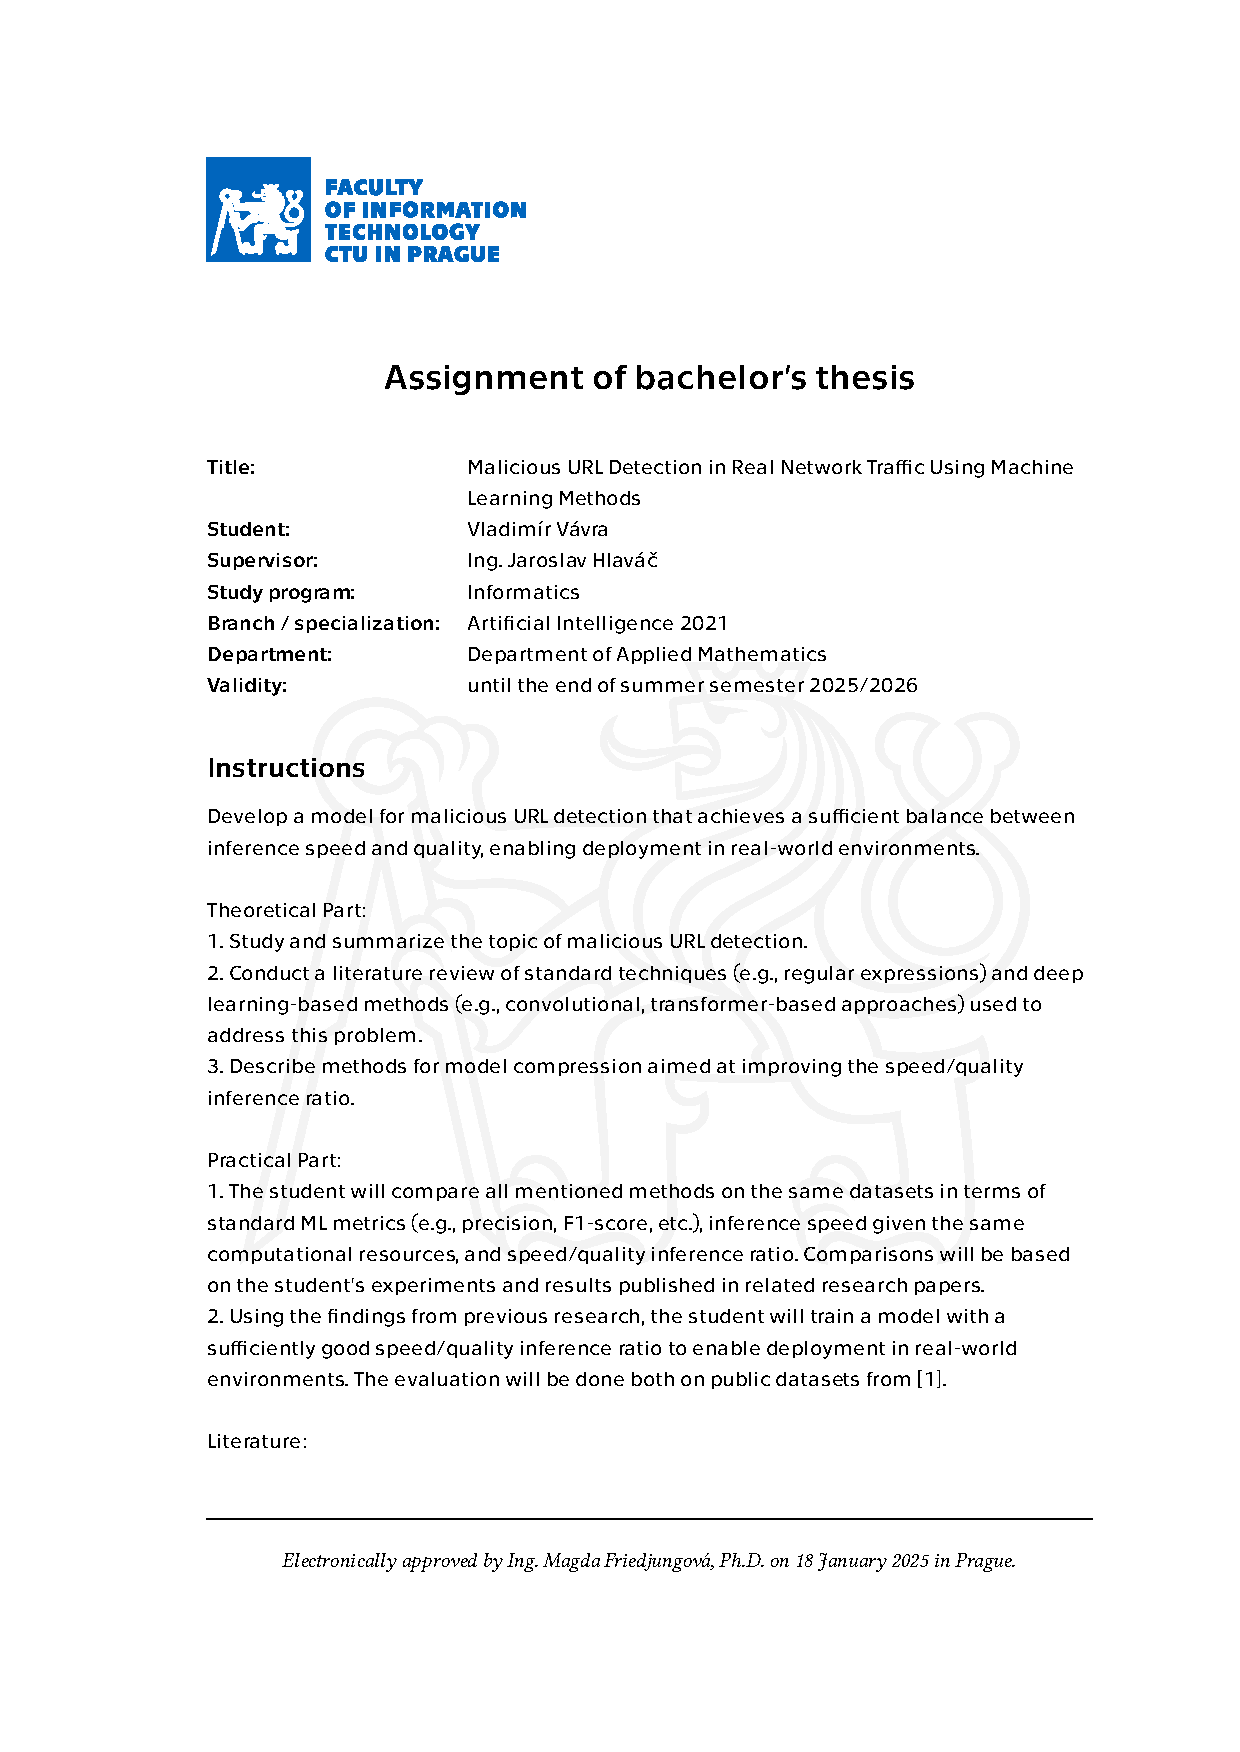
\includepdf[pages={1-}]{vavravl3-assignment.pdf} % replace this file with your thesis assignment generated from ProjectsFIT

\thispagestyle{empty}\maketitle\thispagestyle{empty}\cleardoublepage % do not remove these four commands


\interfootnotelinepenalty=10000
\imprintpage % do not remove this command
\stopTOCentries
%%%%%%%%%%%%%%%%%%%%%%
% list of other contents END
%%%%%%%%%%%%%%%%%%%%%%

%%%%%%%%%%%%%%%%%%%
% ACKNOWLEDGMENT
% FILL IN / MODIFY
% This is a place to thank people for helping you. It is common to thank your supervisor.
%%%%%%%%%%%%%%%%%%%
\begin{acknowledgmentpage}
    I would like to express my gratitude to my thesis supervisor, Ing. Jaroslav Hlaváč, for his guidance and valuable feedback throughout the development of this bachelor's thesis.

    I would also like to thank Cisco Systems for providing the computing resources required to carry out the experiments.
\end{acknowledgmentpage}
%%%%%%%%%%%%%%%%%%%
% ACKNOWLEDGMENT END
%%%%%%%%%%%%%%%%%%%


%%%%%%%%%%%%%%%%%%%
% DECLARATION
% FILL IN / MODIFY
%%%%%%%%%%%%%%%%%%%
% INSTRUCTIONS
% ENG: choose one of approved texts of the declaration. DO NOT CREATE YOUR OWN. Find the approved texts at https://courses.fit.cvut.cz/SFE/download/index.html#_documents (document Declaration for FT in English)
% CZE/SLO: Vyberte jedno z fakultou schvalenych prohlaseni. NEVKLADEJTE VLASTNI TEXT. Schvalena prohlaseni najdete zde: https://courses.fit.cvut.cz/SZZ/dokumenty/index.html#_dokumenty (prohlášení do ZP)
\begin{declarationpage}
    I hereby declare that the presented thesis is my own work and that I have cited all sources of information in accordance with the Guideline for adhering to ethical principles when elaborating an academic final thesis.
    I acknowledge that my thesis is subject to the rights and obligations stipulated by the Act No. 121/2000 Coll., the Copyright Act, as amended. In accordance with Section 2373(2) of Act No. 89/2012 Coll., the Civil Code, as amended, I hereby grant a non-exclusive authorization (licence) to utilize this thesis, including all computer programs that are part of it or attached to it and all documentation thereof (hereinafter collectively referred to as the "Work"), to any and all persons who wish to use the Work. Such persons are entitled to use the Work in any manner that does not diminish the value of the Work and for any purpose (including use for profit). This authorisation is unlimited in time, territory and quantity.

    I declare that I have used AI tools during the preparation and writing of my thesis. I have verified the generated content. I confirm that I am aware that I am fully responsible for the content of the thesis.
\end{declarationpage}
%%%%%%%%%%%%%%%%%%%
% DECLARATION END
%%%%%%%%%%%%%%%%%%%

% Use one of the two following commands. The first prints abstracts+keywords on two pages, the second puts them on one page (if possible). \printonepageabstract can also accept optional argument that specifies a vertical space before both abstracts (the default is 18 mm).
\printtwopageabstract
%\printonepageabstract 

%%%%%%%%%%%%%%%%%%%
% SUMMARY
% FILL IN / MODIFY
% OR REMOVE ENTIRELY (upon agreement with your supervisor)
% (appropriate to remove in most theses)
%%%%%%%%%%%%%%%%%%%
% \begin{summarypage}
% \section*{Summary section}
% 
% \lipsum[1][1-8]
% 
% \section*{Summary section}
% 
% \lipsum[2][1-6]
% 
% \section*{Summary section}
% 
% \lipsum[3]
% 
% \section*{Summary section}
% 
% \lipsum[2]
% 
% \section*{Summary section}
% 
% \lipsum[1][1-8] Lorem lorem lorem.
% \end{summarypage}
%%%%%%%%%%%%%%%%%%%
% SUMMARY END
%%%%%%%%%%%%%%%%%%%

\tableofcontents % do not remove this command
%%%%%%%%%%%%%%%%%%%%%%
% list of other contents: figures, tables, code listings, algorithms, etc.
% add/remove commands accordingly
%%%%%%%%%%%%%%%%%%%%%%
\listoffigures % list of figures
\begingroup
\let\clearpage\relax
\listoftables % list of tables
% \thectufitlistingscommand
\endgroup

\resumeTOCentries
\mainmatter\mainmatterinit % do not remove these two commands
%%%%%%%%%%%%%%%%%%%
% THE THESIS
% MODIFY ANYTHING BELOW THIS LINE
%%%%%%%%%%%%%%%%%%%

\setcounter{page}{1}

\chapter*{Introduction}
This thesis deals with models used for malicious URL (Uniform resource locator) detection. Such models are trained to determine whether a URL points to malicious or benign content using only information from the URL string. The thesis aims to train a model with a higher inference speed than the current baselines while maintaining predictive performance.

The motivation for the thesis stems from the fact that URL string-based models operate in the early stages of the malicious URL detection pipeline. While basic mechanisms like blocklists and allowlists can precede this step, they fail to generalize to newly registered or previously unseen domains. On the other hand, methods for website content analysis can deliver better predictions but are too computationally expensive. URL-string-based models offer a practical middle ground -- they're fast and scalable, making them ideal for quickly filtering out obvious cases. This helps narrow the list of suspicious URLs, so heavier detection methods only need to handle the smaller, high-risk group.

Although this thesis focuses on binary classification, the approach can be extended to multi-class scenarios, predicting specific attack types such as credential phishing or drive-by downloads.

The thesis begins by providing a broader context to the problem of malicious URL detection. This is followed by a summary of related work focusing on existing URL-based detection methods and methods for increasing model speed, such as quantization.

Afterwards, a thorough exploratory analysis was conducted on both public datasets and a private dataset, using real-world data provided by Cisco through the thesis supervisor. This analysis revealed that standard dataset splitting can lead to performance overestimation, as models tend to memorize second-level domains instead of learning generalizable features. A specialized strategy for splitting datasets was used to ensure a more realistic estimation of model performance.

Following this, the BERT-Small~\cite{turc2019} model and selected models from related work were evaluated on the prepared datasets to establish baseline performance for subsequent experiments. To improve inference speed, the thesis adopts two main complementary strategies.

The first focuses on training inherently smaller and faster models while maintaining predictive performance comparable to baseline models. An ablation study was performed on the BERT-Tiny variant to identify better hyperparameter combinations for BERT-based models. Additionally, a novel data augmentation technique, domain masking, was introduced to mitigate over-fitting caused by memorization of domain names during training. Combining these improvements with the BERT-Mini~\cite{turc2019} architecture resulted in outperforming the larger BERT-Small in key evaluation metrics.

The second approach used in the thesis focuses on compressing existing models to increase their inference speed. Different quantization techniques were applied to the BERT-Small and BERT-Mini variants. These experiments showed that substantial speedups can be achieved with minimal impact on detection performance.

Experimental results presented in this thesis show that combining both approaches achieves a trade-off between predictive performance and inference speed.

\chapter{Malicious URL detection}

This chapter focuses on providing a broader context for malicious URL detection (using URL strings only). It begins by defining, in detail, what a URL is and how it is structured. It then describes the types of attacks that attackers can execute using URLs. The next part focuses on what kinds of information can be used to detect the attacks in general, and what kind of information can be used to detect the attacks using only the URL string. The last part then describes, where the model would fit in a real environment.

\section{What Is a URL?}

A URL (RFC 3986~\cite{rfc3986}) (Uniform Resource Locator) defines the address of a resource on the internet. This section provides a detailed overview of the structure of URLs.

A URL consists of multiple components, each serving a specific syntactic and functional role. The general structure of a URL~\cite{rfc3986} is shown in Figure~\ref{fig:url_syntax}, followed by a real-world example with labelled parts in Figure~\ref{fig:url_structure_example}.

\begin{figure}[H]
    \centering
    \wrappedttt{scheme://[user@]host[:port]/path[?query][\#fragment]}
    \caption{General syntax of a URL. The components are shown in square brackets, indicating that they are optional.}
    \label{fig:url_syntax}
\end{figure}

\begin{figure}[H]
    \centering
    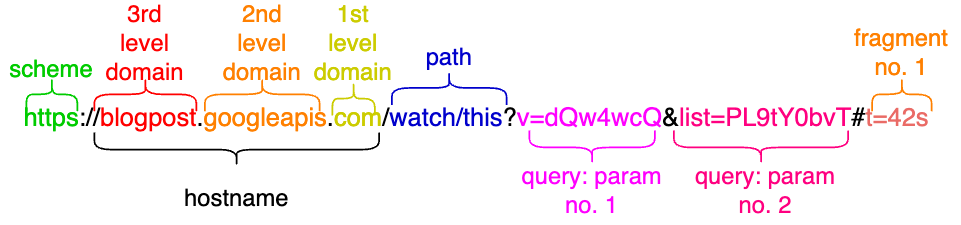
\includegraphics[width=1\textwidth]{images/url_structure_example.png}
    \caption{Example of a URL structure with labelled components}
    \label{fig:url_structure_example}
\end{figure}

Each component of a URL serves a different purpose. Below are the purposes for each section accompanied by a part of a real example depicted in Figure~\ref{fig:url_structure_example}.

\begin{itemize}
    \item \textbf{Scheme:} \wrappedttt{https} indicates the protocol to use. It tells the client (usually a browser) to communicate securely with the server using HTTP over TLS. Common schemes include \wrappedttt{http}, \wrappedttt{https}, \wrappedttt{ftp}, and \wrappedttt{mailto}.
    \item \textbf{User (optional):} Credentials can be embedded in the URL as \wrappedttt{user@host}. For example, \wrappedttt{ftp://admin@ftp.example.com} uses \wrappedttt{admin} as the username. This is uncommon in the modern web and its usage could be a signal of potentially malicious behaviour (this is more explored in the related work section).
    \item \textbf{Hostname:} \wrappedttt{blogpost.googleapis.com} identifies which server should be contacted. It is either an IP address or a DNS-resolvable hostname~\cite{rfc1035}.
    \item \textbf{Path:} \wrappedttt{/watch/this} specifies the location of the resource on the server. Its meaning is interpreted by the server (REST API, file system, etc.). The path is hierarchical and may include multiple segments separated by slashes.
    \item \textbf{Query:} \wrappedttt{?v=dQw4wcQ\&list=PL9tY0bvT} contains URL parameters in key-value pairs. Here, \wrappedttt{v} and \wrappedttt{list} might refer to a video ID and a playlist. Queries allow dynamic interaction with the backend without altering the path.
    \item \textbf{Fragment:} \wrappedttt{\#t=42s} refers to a client-side anchor or setting, such as scrolling to a specific section or timestamp. Fragments are never sent to the server and are interpreted entirely by the browser.
\end{itemize}

\subsection{Hostname}
The hostname component of a URL can take two distinct forms.

The first form is an IP address. IPv4 addresses, as specified in RFC 791~\cite{rfc791}, are represented in dotted-decimal notation, for example \wrappedttt{8.8.8.8}. IPv6 addresses, defined in RFC 8200~\cite{rfc8200}, use a colon-separated hexadecimal format and must be enclosed in square brackets when included in URLs, such as \wrappedttt{[2001:db8::1]}. When an IP address is used as the hostname, DNS resolution is bypassed, and the client connects directly to the specified address.

The second form is a DNS-resolvable domain name, which follows a hierarchical structure. For example, in Figure~\ref{fig:url_structure_example}, the label \wrappedttt{blogpost} is a subdomain of \wrappedttt{googleapis.com}, while \wrappedttt{googleapis} is the second-level domain under the top-level domain \wrappedttt{.com}.

The second-level domain (SLD), such as \wrappedttt{googleapis}, identifies the entity that has registered the domain within a given top-level domain (TLD). Common TLDs include generic domains like \wrappedttt{.com} and \wrappedttt{.org}, as well as country-code TLDs such as \wrappedttt{.cz}. These domains are managed by ICANN (Internet Corporation for Assigned Names and Numbers). The Domain Name System (DNS), as defined in RFC 1035~\cite{rfc1035}, is responsible for resolving domain names to their corresponding IP addresses.

\section{Types of URL-Based Attacks}
\label{sec:types_of_url_attacks}

This section outlines several common types of attacks where the malicious payload or intent is embedded in the URL itself. The selected few that are mentioned here are the most common ones mentioned repeatedly in reports from Webroot 2019 report~\cite{webroot2019} and FBI 2024 report~\cite{fbi2024ic3report} or were present in the datasets used in this thesis.

\begin{itemize}
    \item \textbf{Credential Phishing:} These attacks use deceptive URLs to impersonate legitimate services and trick users into submitting sensitive information like as login credentials or financial details. Attackers often register domains that closely resemble real ones. The key signal that a URL might be leading to a phishing website is that it tries to appear as if it leads to the website it tries to impersonate. According to~\cite{fbi2024ic3report}, a phishing attack in 2024 caused over 70 million USD in losses for US citizens.

    \item \textbf{Drive-by Downloads:} URLs of this type cause the user's browser to automatically download and execute malicious content, typically without user interaction. These may exploit vulnerabilities in the browser or plugins to install malware. They are especially effective if user does not have up-to-date software.

    \item \textbf{Crypto-jacking:} Some URLs lead to pages that execute cryptocurrency mining scripts, consuming the user's computing resources without their consent. This is usually implemented through embedded JavaScript and can be triggered as soon as the page loads.

    \item \textbf{File-less Attacks:} In file-less attacks, the malicious payload is not delivered as a downloadable file, but rather executed directly from memory, often via scripts embedded in the URL itself (e.g., encoded PowerShell, JavaScript, or Bash). These may appear in query strings or path segments and are difficult to detect through traditional signature-based methods.

    \item \textbf{Custom Malicious Content:} Some URLs lead to content that, while not technically malware, is designed to harm users or violate platform policies. This includes links to explicit pornography, scams, illegal downloads, hate content, or violent material. Custom models can be trained to detect these types of URLs, if the organization needs it.
\end{itemize}

\section{Information Usable for Detection}

Multiple types of information can be used to detect whether a given URL is malicious. This thesis proposes a categorization of the information into four groups, similar to the 2017 survey on malicious URL detection~\cite{surveymaliciousfeatures}.

\subsection{Content-based information}
\label{sec:content_based_info}
This information is not at all taken into account for this thesis. It is the information that can be extracted from the content of the page that the URL points to. This includes but is not limited to, the HTML (Hyper-text markup language) content of the page, JavaScript code, and any other resources that are loaded when the page is opened.

Semantic information about the content can be used too. For example, if the content of the page contains content that requires input credentials, it should be more suspicious, because it could be a credential phishing attack. This type of information was usually mined manually by data analysts in the past. However, recent work such as~\cite{koide2025detectingphishingsitesusing} shows that large language models like ChatGPT can process both raw HTML and webpage screenshots to extract high-level semantic cues.

Another type of information that can be extracted from the content of a website is very similar to the content of some high-profile websites. This might indicate that the site is trying to trick users into thinking they are on a some other legitimate website, such as PayPal, while they are in reality going to send their credentials to an attacker. An example of work that tries to leverage this type of information is~\cite{VisualPhishNet}, which uses a triplet Convolutional Neural Network (CNN) to create embeddings of the examined website and compare it against the embeddings of a few legitimate websites.

\subsection{Domain-based metadata}
\label{sec:domain_based_info}
This group consists of every bit of external knowledge about the domain that is present in the URL.

The simplest and most widely used information from this group is the presence of domains on either blocklists or allowlists. Blocklists contain known malicious domains, or IP addresses, which should always be blocked. These are typically maintained by security vendors, threat intelligence services, or community-driven projects like PhishTank~\cite{PhishTank} or OpenPhish~\cite{OpenPhish}. In addition, many organizations maintain their internal blocklists, curated by their Security Operations Center (SOC) teams, based on incidents observed within their networks.

Allowlists, on the other hand, contain trusted URLs that should always be allowed. These can include popular websites, internal company resources, or other trusted domains.

The information about the domain does not have to be absolute -- malicious or benign but can be expressed as a reputation score. Different ranking scores like Google PageRank~\cite{Page1998PageRank} (or similar, that are available publicly) can be used to determine the quality of the domain.

Metadata such as the age of the domain and WHOIS~\cite{whois} registration information has been widely used in prior work~\cite{surveymaliciousfeatures}. For example, domains registered only days before being used are more likely to be malicious~\cite{surveymaliciousfeatures}.

Another type of information also discussed in~\cite{surveymaliciousfeatures}, is whether the domain attempts to mimic a well-known domain. For example, if the domain is \wrappedttt{pay-pal.com} instead of \wrappedttt{paypal.com}, it may be trying to trick users into thinking that they are on the legitimate site. The crucial part here is the inclusion of certain information about the domain the URL tries to impersonate. Should the impersonated domain be a very popular one and hackers might want to target it because of its content (banking, credentials, ...), the URL should be considered more suspicious.

This is not limited to SLDs if the domain is \wrappedttt{paypal.malicious.com}, it may be trying to impersonate the legitimate site as well. Special features, such as Levenshtein distance can be used to determine how similar the domain is to the legitimate one in terms of edit distance.

Another way to determine the similarity try to detect the homoglyph attack, where the attacker uses visually similar characters to trick users into clicking on a malicious link. For example, the letter "o" in the domain \wrappedttt{g00gle.com} is replaced with two zeros.

\subsection{URL-string Based Information}
URL-string-based information refers to any feature that can be extracted directly from the URL string itself, without requiring external lookups or content analysis. This includes structural properties, handcrafted features, specific characters or keywords, semantic hints from query parameters, and common domain name obfuscation patterns.

One example of such information is the presence of the \wrappedttt{@} character. In URL syntax, any part of the string preceding \wrappedttt{@} is treated as user information and ignored during host resolution. For instance, the URL \wrappedttt{http://legitimate.com@malicious.com} appears to reference \wrappedttt{legitimate.com}, but in reality, the browser connects to \wrappedttt{malicious.com}.

Attackers may also exploit excessively long URLs to conceal malicious content. For example, a URL like \wrappedttt{http://example.com/secure/account/update/redirect?next=aHR0cHM6Ly93d3cucGF5cGFsLmNvbS9sb2dpbg==} can seem legitimate at first glance, yet contains a redirect parameter that points to a malicious destination hidden deep within the URL.

Another obfuscation technique in this category known as a homoglyph attack exploits visually similar characters to disguise malicious URLs. Attackers register domains using Unicode characters that closely resemble legitimate ones, tricking users into believing the URL is safe. While users typically see URLs rendered in Unicode, only ASCII characters are transmitted over the network, as specified in RFC 3986~\cite{rfc3986}. Unicode characters are transformed into ASCII-compatible encodings before transmission and later rendered back into a user-friendly form by browsers. Although the visual similarity is lost after encoding, text-based models can still detect such attacks by learning to recognize uncommon character patterns or domain name irregularities that often accompany these manipulations.

Exhaustive research is conducted on this type of information in the related work chapter, as it is the only source of information models trained in this thesis use.

\section{Detection Pipeline}
\label{sec:real_world_pipeline}
This section outlines the overall architecture of a typical malicious URL detection pipeline. Although the primary focus is on large-scale threat intelligence services, it is important to note that optimizing models for size and inference speed can unlock entirely new deployment scenarios (for example deployment directly in the web browser).

In a standard threat intelligence setting, clients submit URLs they wish to verify for potential malicious activity. These requests can easily reach tens of millions per day. To manage such volumes, a multi-stage architecture with progressively more computationally expensive models is used. Each layer attempts to resolve as many URLs as possible before the next step.

\begin{figure}[H]
    \centering
    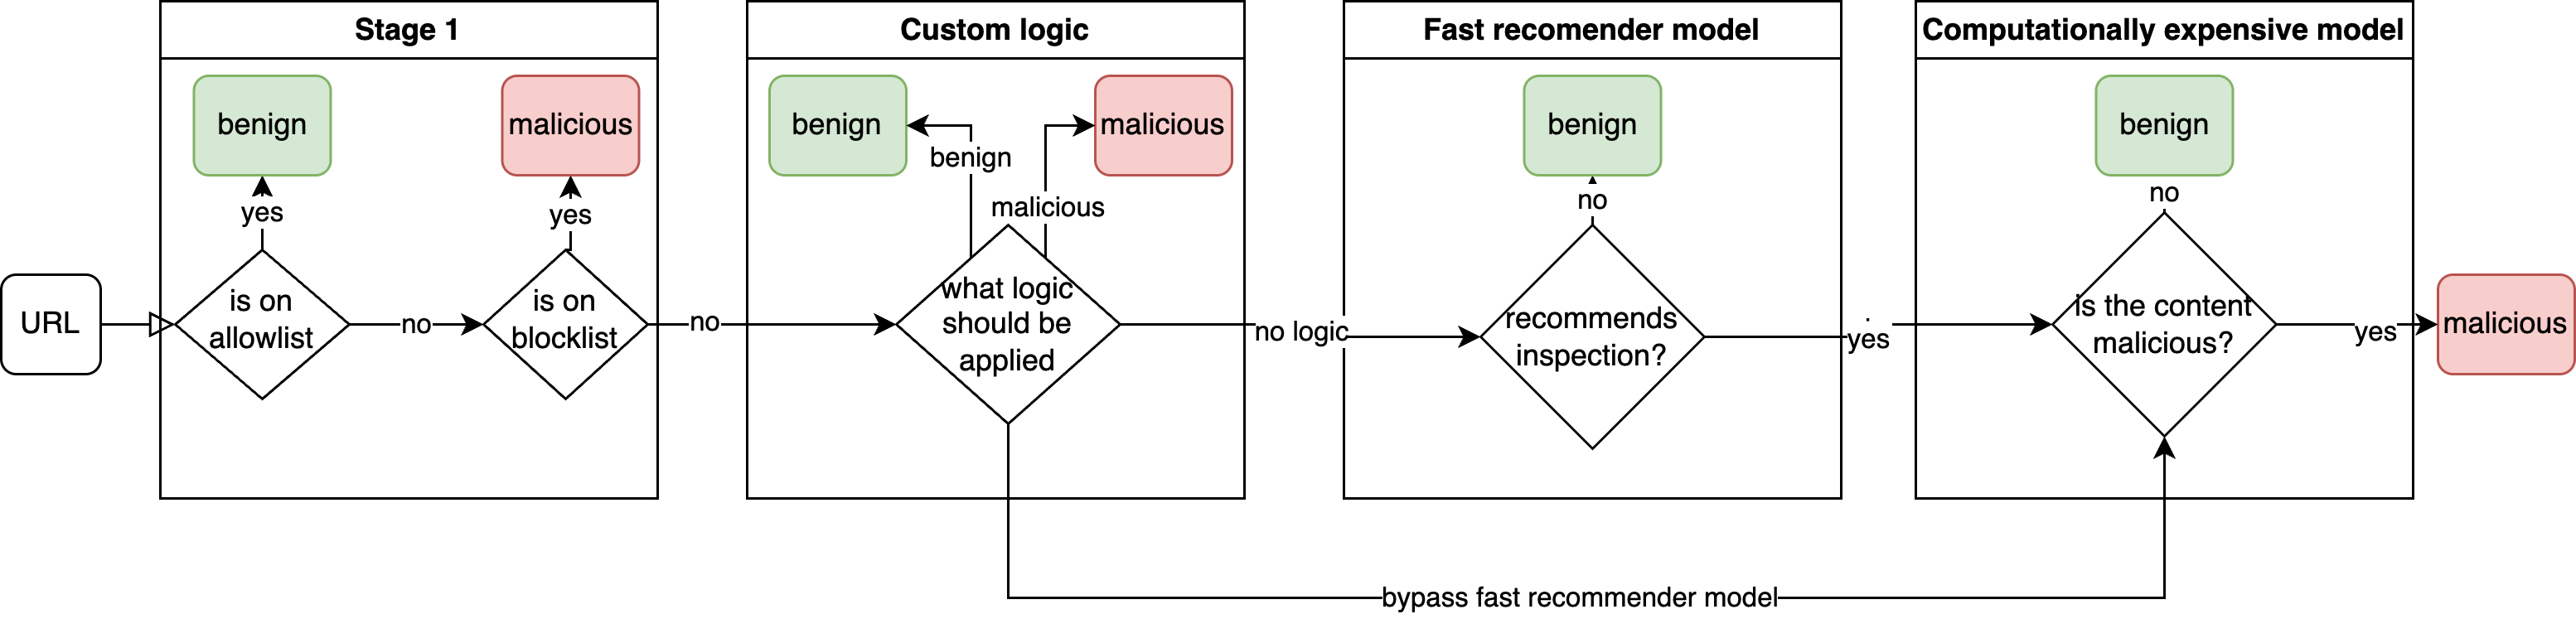
\includegraphics[width=1\textwidth]{images/pipeline_diagram.png}
    \caption{Example of a URL detection pipeline}
    \label{fig:detection_pipeline}
\end{figure}

The typical detection pipeline consists of the following stages, which can be seen in~\ref{fig:detection_pipeline}:
\begin{itemize}
    \item \textbf{Blocklist/Allowlist} -- The first stage filters out URLs based on allowlists of known benign domains and blocklists of known malicious domains. This step quickly discards a significant portion of URLs without further processing. It can be continuously updated based on previous model results.

    \item \textbf{Custom Pre-Filtering} -- Domain-specific rules can be applied in this stage. For example, URL shorteners such as \wrappedttt{bitly.com}~\cite{bitly} generate compact links that redirect to a final destination. These services obscure the actual target URL with a short, seemingly random one, which gives the string-based model no information to classify it correctly. Therefore, a custom logic should automatically flag such URLs for deeper inspection in later pipeline stages.

    \item \textbf{Fast Recommender Model} -- At this stage, a lightweight model processes large volumes of URLs (thousands per second) and flags those that are likely to be malicious. URLs deemed suspicious are passed to the next stage for further analysis, while the rest are discarded.

    \item \textbf{Computationally Expensive Model} -- In this stage, the model uses information from Sections~\ref{sec:content_based_info} about content and from~\ref{sec:domain_based_info} about domains.
\end{itemize}

The model developed in this thesis is intended for the Fast Recommender Stage, where the primary objective is to identify as many malicious URLs as possible, even at the cost of increased false positives -- though this must remain within reasonable limits, as each detection triggers an expensive computational in the next stage.

\chapter{Related work}
\label{sec:related_work}
This chapter provides overview of the existing methods that are directly related to the topic of the thesis. This includes techniques for malicious URL detection based on generalizable string information and methods for model compression.

\section{Manual Feature Engineering}
\label{sec:man_feat_eng}
One of the simplest approaches to malicious URL detection is to extract a set of manually engineered features from the URL string and train a standard feature-based classifier. This strategy is followed in~\cite{lexicalFeaturesModels}, and a broader overview of such features is presented in the survey by~\cite{surveymaliciousfeatures}.

Features that these papers mention can be summarized as follows:
\begin{itemize}
    \item \textbf{From the whole URL} -- length; the number of semicolons, underscores, question marks, equals, ampersands; digit to letter ratio; entropy of the string
    \item \textbf{SLD} -- contains IP; length; number of digits; number of non-alphanumeric characters; number of hyphens; number of @s
    \item \textbf{TLD} -- presence in suspicious list
    \item \textbf{Subdomain} -- number of dots; number of subdomains
    \item \textbf{Path} -- number of '//'; number of subdirectories; presence of '\%20'; presence of uppercase directories; presence of single-character directories; number of special characters; number of zeroes; ratio of uppercase to lowercase characters
    \item \textbf{Query parameters} -- total length; number of queries; number of variables; presence of encoded scripts (e.g., Base64)
    \item Presence of specific \textbf{keywords} -- (e.g., \texttt{login}, \texttt{secure}, \texttt{cmd=}, \texttt{redirect=}, \texttt{confirm}, \texttt{update}, \texttt{verify}, \texttt{account})
\end{itemize}

These features are extracted using a combination of URL parsing, regular expressions, and custom logic. Once extracted, they are fed into a classifier. In~\cite{lexicalFeaturesModels}, models such as logistic regression, XGBoost, and Naive Bayes were used.

No single feature is sufficient to identify a malicious URL definitively. Therefore, implementing a lightweight rule-based system (e.g., using regexes) to pre-filter URLs before the main classifier and gain speedup would degrade predictive performance significantly.

The main advantages of feature-based models are that they are computationally efficient, easy to train and highly interpretable. However, the attackers can adapt their URLs to evade detection by modifying the URL structure or using obfuscation techniques that the features do not cover. This generalization problem is obvious in the keywords features, where the model is trained on a specific set of keywords, and when new keywords appear, or their obfuscated versions are used, the model fails to detect them. This drives the need for more generalizable models based on deep learning.

Nevertheless, the rise of deep learning models does not invalidate the utility of handcrafted features. Certain information, such as URL length, frequency of characters, or the structure of components, is often better represented explicitly. A hybrid approach can be beneficial, where handcrafted features are combined with outputs from a deep learning model. One common strategy is to use the output of the deep model as an input feature for a traditional classifier, a technique known as stacking.

\section{Deep learning-based models}
\label{sec:dl_models}
Unlike feature-based models, the input to deep learning models is the raw URL string. The model learns to extract relevant features from the data during training. This approach allows model to learn more generalizable features, which are not easily captured by handcrafted features, especially in the interaction of semantic and syntactic information.

One of the earliest deep learning models designed specifically for URL-based malicious detection is URLNet~\cite{URLNet}. It uses a dual-branch convolutional neural network (CNN) architecture: one branch processes the URL at the character level and the other at the word level. The character-level branch focuses on patterns such as obfuscation through character substitutions, while the word-level branch targets higher-level structural and semantic patterns by embedding words that are extracted using delimiters like dots or slashes. Both branches are trained jointly in an end-to-end fashion, and their outputs are concatenated and passed through fully connected layers for final classification.

Another example would be a model from GramBeddings~\cite{GramBeddings} paper. Aside from the model, the paper also introduces a new dataset, which is also used in this thesis for experiments. Its description is provided in the dataset Section~\ref{sec:dataset_descriptions}. The model learns embeddings for the most common n-grams (group of n consecutive characters), which are chosen based on dataset statistics and then uses CNN, LSTM (Long short-term memory) and attention mechanisms for classification. Multiple values of $n$ are used to capture different ranges of local context.

Many other deep learning-based models have been proposed, however, they were all recently overshadowed by transformer-based models, therefore other non-transformer models are not discussed in detail.

\section{Transformer-based models}
Transformer-based~\cite{AttentionIsAllYouNeed} models have achieved state-of-the-art results in many natural language processing tasks, including malicious URL detection.

\subsection{BERT}
As demonstrated by the 2021 paper URLTran,~\cite{URLTran}, fine-tuning encoder transformers like BERT~\cite{BERT} or RoBERTa~\cite{RoBERTa} on URL classification tasks has proven very effective.

Before running the model, the input text is tokenized using WordPiece~\cite{wordpiece} tokenizer, which splits words into subword units. This allows the model to handle out-of-vocabulary words and reduces the vocabulary size. The tokenizer also adds special tokens to the input sequence, such as [CLS] for the classification of the whole sentence and [SEP] for segment separation.

The input to BERT is a sequence of tokens formatted as:
$$
    \text{[CLS]},\ t_1,\ t_2,\ \dots,\ t_n,\ \text{[SEP]}
$$
Where [CLS] is a special classification token, and [SEP] marks the end of a single sentence or separates two segments.

Unlike traditional unidirectional models, BERT is bidirectional -- it learns contextual representations by attending to both the left and right of every token at every layer. Since the task of malicious URL only only requires classification, not generation, encoder only models are sufficient.

For example, consider the URL example from~\cite{URLTran}:

\begin{table}[H]
    \centering
    \renewcommand{\arraystretch}{1}
    \resizebox{\textwidth}{!}{
        \begin{tabular}{ll}
            \toprule
            \textbf{Original URL}       & \texttt{secure.bankofamerica.com/login/sign-in/signOnV2Screen.go}                                                                                                                \\
            \midrule
            \textbf{Tokenized Sequence} &
            \texttt{[CLS]}, \texttt{secure}, \texttt{.}, \texttt{bank}, \texttt{\#\#of}, \texttt{\#\#ame}, \texttt{\#\#rica}, \texttt{.}, \texttt{com}, \texttt{/}, \texttt{log}, \texttt{\#\#in}, \texttt{/},             \\
                                        & \texttt{sign}, \texttt{-}, \texttt{in}, \texttt{/}, \texttt{sign}, \texttt{\#\#on}, \texttt{\#\#v}, \texttt{\#\#2}, \texttt{\#\#screen}, \texttt{.}, \texttt{go}, \texttt{[SEP]} \\
            \bottomrule
        \end{tabular}}
    \caption{Example of WordPiece tokenization applied to a URL.}
    \label{tab:tokenization_example}

\end{table}

The tokens are converted to embedding vectors using a learned embedding matrix. Learned positional embeddings can be added~\cite{AttentionIsAllYouNeed} because transformer architecture is permutation invariant.

These embeddings are then fed into the BERT model, whose architecture can be seen in Figure~\ref{fig:transformer}.

\begin{figure}[H]
    \centering
    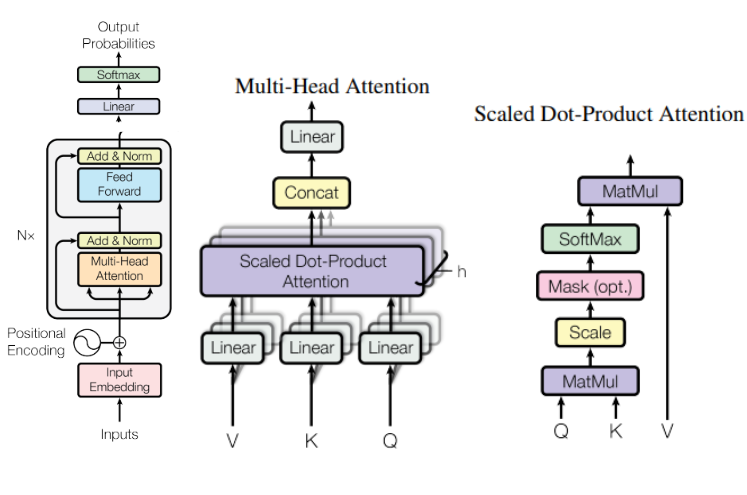
\includegraphics[width=0.9\textwidth]{images/transformer.png}
    \caption{Illustration of an encoder-only transformer architecture. Images are from~\cite{AttentionIsAllYouNeed}. On the left, the entire transformer architecture is shown. In the middle, a multi-head attention block on the left is shown. On the right, scaled-dot-product attention from the middle image is described in detail.}
    \label{fig:transformer}
\end{figure}

It consists of a stack of $N$ identical encoder layers, each containing two main components: a multi-head self-attention mechanism and a feed-forward neural network. Each of these components is followed by layer normalization and residual connections. The input to the scaled-dot-product is a tensor of shape \textit{(batch\_size, sequence\_length, embedding\_dimension)} obtained by multiplying previous layer representations by learned attention matrices. The output is a tensor of the same shape, which is then passed to the feed-forward network.

The self-attention layer provides contextual information to individual token embeddings, and the feed-forward network applies a non-linear transformation to the output of the self-attention layer. More on how the transformers work can be found in~\cite{AttentionIsAllYouNeed,RoBERTa}.

The output used for classification of malicious URLs is then obtained by taking the embedding of the [CLS] token from the last layer of the transformer and passing it through a linear layer with softmax activation function. The output is a probability distribution over the classes, which can be interpreted as the model's confidence in each class.

\subsection{Training strategies}
The models used in URLTran~\cite{URLTran} use pre-trained BERT and RoBERTa models, which are fine-tuned on the target task. The pre-training process involves training the model on a large corpus of text using two tasks: masked language modelling (MLM) and next sentence prediction (NSP).

This allows the model to use semantic knowledge about the keywords in the URL. By fine-tuning the model on the URL dataset, it then strives to learn the specific patterns unique to URLs.

The model can also be pre-trained directly on the URL corpus. This approach is used, for example, by~\cite{urlbert}. The positive aspect of this approach is that the model learns potentially better tokenization for the URL strings, which can be beneficial for the task. On the other hand, it loses the general knowledge about the language, which can be useful for the task because of the presence of specific keywords in the URLs, as mentioned earlier.

Different data augmentation techniques are mentioned in~\cite{URLTran} to learn specific types of attacks. This way, the dataset size can be artificially increased. The first technique is parameter reordering. The second focuses on splitting domain names into words and inserting hyphen characters in between them. The third technique tries to target homoglyph attacks by replacing characters with similar-looking ones.

\subsection{Other architecture improvements}
This sub-section outlines approaches that are not used in this thesis but are proposed as potential directions for future work.

Improvements to the original BERT architecture have been proposed, one of the most notable being CharBERT~\cite{charbert}. This model combines standard subword-level embeddings with additional character-level information using a bidirectional GRU, fusing both representations. Since malicious URLs often vary at the character level, this method may provide valuable information.

One paper applying this idea to malicious URL detection is~\cite{TransURL}, which builds on CharBERT and introduces several enhancements. Although it claims state-of-the-art results, the paper lacks direct comparison with other transformer-based models and uses an evaluation protocol susceptible to domain over-fitting (as discussed in the dataset chapter). A reevaluation of the model would be necessary, and if it proves superior to standard BERT, model distillation could be a promising next step to improve the speed-quality trade-off.

\section{Methods for model compression}
\label{sec:model_compression_methods}

This chapter explores the second approach to improving the speed-quality ratio mentioned in the introductory chapter. Rather than selecting a smaller model from the beginning, this approach focuses on transforming a larger model into a faster version by using model compression methods.

Several existing methods are presented in terms of how they work and how they can be implemented. A brief discussion is included for each method to justify its use or omission in the experimental work.

\subsection{Quantization}

Quantization is a concept that extends beyond the field of machine learning. It generally refers to the process of mapping a large set of input values to a smaller, discrete set.

In the context of machine learning, the purpose of quantization is to map values needed to perform operations of the model from high-precision format (e.g., Float32~\cite{ieee754}) to lower-precision format (e.g., Int8, Float16). The operation is then performed using the lower-precision format, which is faster (if the target hardware supports it) and requires less memory both at runtime and for storing the model. The information from these sources was used for writing this Section~\cite{quantization_whitepaper, nvidia_whitepaper}.

To better understand quantization, consider the example of matrix-vector multiplication that is present in most neural networks. The operation can be expressed as:
\begin{equation}
    y = Wa + b
\end{equation}
where $W$ is the weight matrix, $a$ is the input vector, $b$ is the bias vector, and $y$ is the output vector. This operation, such as all other operations in a model, requires two types of values, which need to be quantized in different ways:
\begin{itemize}
    \item \textbf{Weights} -- These are the parameters of the operation learned during training. They are fixed during inference. In this case, $W$ and $b$ are weights.
    \item \textbf{Activations} -- These are the intermediate outputs of the operation, which depend on the input data. They change for each forward pass. In this case, $a$ and $y$ are activations.
\end{itemize}

\subsubsection*{Float16 quantization}

Float16 (also known as FP16) is a reduced-precision floating-point format that uses 16 bits to represent numbers. It retains the same structural components as Float32 -- a sign bit, exponent, and mantissa, but with fewer bits: 1 for a sign, 5 for the exponent, and 10 for the mantissa. This makes it more memory -- and compute-efficient than Float32 while still being capable of representing a wide dynamic range.

Unlike Int8 quantization, which requires all values to be mapped into a fixed integer range, Float16 quantization allows dynamic range representation because of the ability of floating-point numbers of use exponent to represent both very small and very large numbers.

When quantizing to Float16, the only thing that needs to be done is therefore a simple conversion of the Float32. The model then can use Float16 at runtime instead of Float32 without any additional changes.

\subsubsection*{Int8 quantization}

Unlike the previous example, Int8 quantization requires a more complex process. The goal is to map the original float values to a smaller fixed integer range, typically from -128 to 127 for signed integers. The mapping is typically done for each tensor separately. Alternative approach are to quantize by parts of the tensor, for example by rows.

The especially problematic part is that the Float32 tensor can have a very wide range of values, while the Int8 representation can only represent 256 discrete values. This means that the quantization process must carefully choose how to map the float values to the Int8 range. If done poorly, the majority of values in the tensor may be mapped outside of this range and clipped, or in the other case, the majority of values may be mapped to a single value, losing important information.

The quantization process can be expressed mathematically as follows:

\begin{equation}
    q = \text{round}\left(\frac{x}{s}\right) + z
    \label{eq:quantize}
\end{equation}
\begin{equation}
    \hat{x} = s \cdot (q - z)
    \label{eq:dequantize}
\end{equation}

Here:
\begin{itemize}
    \item $x$ is the original float value,
    \item $q$ is the quantized integer value,
    \item $s$ is the scale factor (a positive real number),
    \item $z$ is the zero-point (an integer that aligns 0 in float to an integer in the quantized domain).
\end{itemize}

Based on choosing the values of $z$, there are two main strategies. The first one is asymmetric quantization, which allows the zero-point $z$ to be non-zero, which is helpful for values that do not centre around, especially activations.

The second one is symmetric quantization, which assumes that the float range is symmetric around zero. In this case, $z = 0$, and only the scale $s$ needs to be calculated. This is much more efficient as described in~\cite{nvidia_whitepaper}. Often, accelerators support only this type of quantization.

\subsubsection*{Static vs. dynamic quantization}

The weights of the model are static and do not change during inference. Therefore, the quantization coefficients can be computed offline and also remain unchanged, since the range of tensors is known ahead of time.

That is not the case for activations, which are dependent on the input tensor. There are two main strategies for computing these parameters for activations: static and dynamic quantization. The difference between them lies in \textbf{when} the quantization parameters ($s$, $z$) are calculated and \textbf{what data} is used to compute them.

\textbf{Static quantization} computes scale and zero-point values ahead of time before inference. This is done using a calibration dataset, which is a representative subset of the training or validation data. The quantization parameters are derived from the observed distributions of activations and remain fixed during inference. Because these parameters are known in advance, static quantization allows for faster inference.

The simplest approach for computing the scale and zero-point is based on the minimum and maximum values of the activation or weight tensor:
$$
    s = \frac{x_{\text{max}} - x_{\text{min}}}{q_{\text{max}} - q_{\text{min}}}, \quad z = \text{round}\left(q_{\text{min}} - \frac{x_{\text{min}}}{s}\right)
$$
However, this \textbf{min-max} method is sensitive to outliers, which can lead to overly large quantization ranges and poor resolution for most values.

To address this, more sophisticated strategies are often used:

\begin{itemize}
    \item \textbf{Percentile-based calibration} clips the extreme values and uses a predefined percentile range (e.g., 99.9\%) to compute $x_{\text{min}}$ and $x_{\text{max}}$. This improves precision by ignoring rare outliers.
    \item \textbf{Entropy-based calibration} selects the quantization range that minimizes the Kullback-Leibler divergence between the original (float) distribution and the quantized distribution.
    \item \textbf{MSE-based calibration} minimizes the mean squared error between the original and quantized tensors.
\end{itemize}

\textbf{Dynamic quantization}, on the other hand, computes quantization parameters on-the-fly during inference. Only weights are quantized offline. When activations are encountered during inference, their scale and zero-point are computed based on the actual input batch.

\subsubsection*{Post-training quantization vs. quantization-aware training}

Once the quantization scheme is chosen, the quantized model can be obtained either through post-processing or during training.

\textbf{Post-training quantization (PTQ)} applies quantization after the model has been fully trained. The model's weights and (optionally) activations are quantized, either statically or dynamically. This approach is fast and easy to apply but may lead to reduced predictive performance.

\textbf{Quantization-aware training (QAT)} addresses this by simulating quantization during training. Fake quantization operators are inserted into the computation graph, allowing the model to adapt to quantization noise. This typically results in higher predictive performance, as the model learns to be robust to low-precision representations. However, QAT requires retraining and is more computationally expensive.

\chapter{Datasets}
In this chapter, a description of the datasets used in the experiments is provided. Four public datasets, one private dataset, and one additional dataset constructed by merging several public datasets were used in this thesis. In the first section of this chapter, the datasets are presented individually. This includes information about their size, content (whether they contain only phishing URLs or also other types of malicious URLs), and how the data was collected. The next section presents the exploratory data analysis performed on the datasets, highlighting both the methods used and the key insights obtained.

\section{Individual Dataset Descriptions}
\label{sec:dataset_descriptions}

\subsection{GramBeddings}
The dataset consists of approximately 800,000 URLs, evenly split between phishing and benign URLs. It was developed as a part of the paper~\cite{GramBeddings}.

The data has been collected over a long-term period (May 2019 -- June 2021), with weekly sampling intervals. After all data was collected, the authors post-processed the URLs to filter them with almost identical domain information.

The phishing URLs were collected from PhishTank~\cite{PhishTank} and OpenPhish~\cite{OpenPhish}. These online services collect, verify, and provide phishing URL lists. Anyone can use their website or API to check whether a given URL is classified as phishing. PhishTank, operated by Cisco Talos, allows users to report and validate phishing sites, maintaining a community-driven blocklist. Since data is labelled by humans, it achieves high accuracy but takes longer to classify phishing URLs. OpenPhish is an automated service that continuously crawls and analyzes phishing URLs using machine learning methods, offering free and commercial threat feeds.

Benign URLs were collected using a custom web crawler. In the beginning, it downloaded the content of the 20 most popular websites in each country. Then, all links from these websites are extracted and filtered to remove duplicates and similar URLs. Now, the content of websites behind these URLs is downloaded and processed in the same way. This process is repeated until the desired number of benign URLs is reached, which in this case was 2 million. A subset of 400,000 URLs was randomly selected to match the number of phishing URLs. This method should produce a diverse set of benign URLs as it is expected that popular websites are not phishing sites themselves, nor do they contain links to phishing sites.

\subsection{Mendeley}
The Mendeley dataset~\cite{Singh2020Mendeley} comprises 1,561,934 URLs, exhibiting a substantial class imbalance with 1,526,619 benign URLs and 35,315 malicious URLs, leading to a 1:43 skew in favour of benign URLs. Unlike the GramBeddings dataset, this one marks every category of harmful URLs described in previous sections as malicious, not just phishing. The original dataset contains more information than just URL and label, but for the purposes of this study, only these two fields were used.

The dataset was constructed using a specialized crawler designed to crawl more malicious URLs than traditional crawlers. The labels are then classified as either benign or malicious using Google Safe Browsing API~\cite{GoogleSafeBrowsing}, which is a similar service as PhishTank and OpenPhish mentioned earlier. The data was collected for an unknown period of time up to May 2020.

The Mendeley dataset is closer to real-world web distributions, where malicious URLs are significantly outnumbered by benign ones. This imbalance presents challenges in training machine learning models, as classifiers may become biased towards the majority class. On the other hand, it makes it a good benchmark for evaluating model performance in realistic scenarios. However, the number of malicious URLs is rather small compared to all other datasets, especially the private dataset~\ref{sec:private_dataset}, which is imbalanced too but has significantly more malicious samples (283,616).

\subsection{Kaggle Multiple}
This dataset~\cite{SiddharthaMaliciousURLs} is used for a multi-class classification and consists of 651,191 URLs categorized into four classes:

\begin{itemize}
    \item 342,651 benign (safe) URLs —- Primarily collected from the ISCX-URL-2016 dataset~\cite{ISCX-URL-2016}. It was collected in 2016.
    \item 18,857 malware URLs -- Sourced from a specialized malware dataset and the ISCX-URL-2016 dataset.
    \item 76,252 defacement URLs —- Extracted from the ISCX-URL-2016 dataset. The defacement attack \cite{wikipedia2024defacement} involves altering the content of a legitimate website to display unauthorized or malicious content. This is often done through SQL injection or other vulnerabilities in the web application. Since the website is legitimate and only the content is altered, the URL itself does not have enough information to detect this type of attack. Therefore, all of the URLs with this class are removed from the dataset.
    \item 75,135 phishing URLs —- Gathered from multiple sources, including PhishTank and PhishStorm~\cite{Marchal2014PhishStorm}. PhishStorm contains data up to 2014. The collection period for the PhishTank data is unspecified.
\end{itemize}

This dataset is used in Section~\ref{sec:multi_class_experiment}, which checks whether the URL-string-based models can be used for multi-class classification after domain-aware folding introduced in Section~\ref{sec:train_test_split} is applied.

\subsection{Kaggle binary}
The Kaggle binary dataset~\cite{KaggleBinaryDataset} consists of 632,503 URLs, evenly distributed between 316,252 benign URLs and 316,251 malicious URLs. Because of the way the dataset was constructed, it can be assumed that URLs labelled as malicious are pointing to either phishing, malware or defacement. The dataset was constructed by combining and preprocessing data from two separate publicly available Kaggle datasets:
\begin{itemize}
    \item First dataset -- Contains 450,176 URLs, with 77\% benign and 23\% malicious URLs. Malicious data were collected using PhishTank and an unknown number of other services. They may or may not include non-phishing malicious URLs. The last update for this dataset was in 2019.
    \item The second dataset -- Kaggle Multiple datasets described earlier. Initially, all URLs labelled as phishing, defacement, and malware were added to this dataset under the "malicious" label. All URLs labelled as defacement in the previous dataset must also be manually removed from this one to ensure consistency with the chosen detection approach.
\end{itemize}

\subsection{Private Dataset}
\label{sec:private_dataset}
This dataset was provided by the supervisor and consists of real-world data from the customers that want to check, whether URL is malicious or not. It was collected in August 2024 by Cisco Talos. It consists of 2,836,160 URLs, with 2,552,544 labeled as benign (90.0\%) and 283,616 labeled as malicious (10.0\%). The dataset was created by down-sampling benign URLs from an even more imbalanced distribution to make training focus more on the malicious samples.

Unlike the public datasets, this dataset has undergone pre-filtering, meaning many obviously benign or trivially malicious URLs were excluded before labeling. As a result, the classification on this dataset is more difficult, since the remaining examples tend to be more ambiguous or sophisticated.

Due to confidentiality restrictions, the private dataset cannot be included in this thesis. However, experimental evaluations performed on this dataset are provided and discussed in later chapters. This offers insights into how the model performs on real-world data and illustrates how well evaluation results obtained on public datasets translate to real-world scenarios.

\subsection{Joined Dataset}
A new dataset was created by merging the GramBeddings, Kaggle Binary, and Mendeley datasets. The goal was to expose the model to a wider variety of URL patterns and malicious behaviors while addressing the shortcomings of individual datasets -- GramBeddings and Kaggle Binary are balanced but small, while Mendeley lacks sufficient malicious samples.

Although combining datasets introduces variations in data distributions, this approach aligns with the original public datasets, which were themselves assembled from multiple other datasets and sources.

After preprocessing, the final dataset contains 2,862,060 URLs: 2,194,899 labeled as benign (76.69\%) and 667,161 labeled as malicious (23.31\%). A total of 8,296 URLs (approximately 0.29\%) were dropped during preprocessing due to deduplication and filtering.

\section{Preprocessing}
This section describes the key preprocessing steps applied to the raw public datasets to prepare them for training and evaluation. The private dataset was already preprocessed prior to use and, therefore, required no additional modifications. Everything described here is present in \texttt{data\_preprocessing.ipynb} notebook.

\subsection{Conflicts and Duplicates}
A label conflict arises when the same URL is duplicated and is assigned different labels, either within a single dataset or across multiple datasets. No such conflicts were detected in Kaggle Binary, Kaggle Multiple, or GramBeddings. However, some were found in the Mendeley dataset, likely due to changes in the Google Safe Browsing API responses, initially misclassifying certain URLs and later returning corrected labels upon re-evaluation.

Since no dataset provides timestamps, it is impossible to tell which label is more recent or accurate. All conflicting entries were therefore removed globally. In total, 215 records (105 unique URLs) were deleted -- mostly from Mendeley (195), with smaller contributions from Kaggle Binary (12), Kaggle Multiple (5), and GramBeddings (3).

Aside from these conflicts, there are no duplicates within dataset in GramBeddings, Kaggle Binary, or Kaggle Multiple. However, for Mendeley, 3.05\% of all records are duplications. All of them are removed from the dataset.

When joining the GramBeddings, Kaggle Binary, and Mendeley datasets to create the Joined dataset, 8,296 URLs (0.28\%) were found to be shared between multiple datasets. No URL appears in all three of them. Additionally, only two URLs are shared between the private dataset and any of the public datasets.

\subsection{Train-Test Split}
\label{sec:train_test_split}
The majority of papers in the related work use a simple random split strategy, such as an 80/20 or 90/10 train-test split. However, this leads to unrealistic evaluations. The vast majority of URLs with the same second-level domain in these datasets are either entirely benign or entirely malicious, allowing models to achieve high predictive performance by memorizing domain labels rather than learning generalizable patterns.

Table~\ref{tab:sld_label_distribution} confirms this issue, showing that in nearly all datasets, over 98\% of second-level domains are associated exclusively with either benign or malicious URLs.

\begin{table}[H]
    \centering
    \renewcommand{\arraystretch}{1.2}
    \resizebox{\textwidth}{!}{
        \begin{tabular}{lccc}
            \toprule
            \textbf{Dataset} & \textbf{100\% Malicious} & \textbf{100\% Benign} & \textbf{Mixed Labels} \\
            \midrule
            GramBeddings     & 29.34\%                  & 70.32\%               & 0.34\%                \\
            Kaggle Binary    & 53.63\%                  & 44.77\%               & 1.60\%                \\
            Kaggle Multiple  & 31.12\%                  & 66.03\%               & 2.85\%                \\
            Mendeley         & 2.36\%                   & 97.50\%               & 0.13\%                \\
            Private          & 4.71\%                   & 94.93\%               & 0.36\%                \\
            Joined           & 15.31\%                  & 82.94\%               & 1.75\%                \\
            \bottomrule
        \end{tabular}
    }
    \caption{Distribution of second-level domains by label purity. "Mixed Labels" indicates domains that contain both benign and malicious URLs. For Kaggle Multiple, everything non-benign is considered malicious.}
    \label{tab:sld_label_distribution}
\end{table}

To enable more reliable evaluation, in this work, the dataset is split so that no second-level domain appears in both the train and test set. More generally, the data is partitioned into N folds, ensuring that all URLs sharing the same domain are assigned to the same fold. This thesis uses 5-fold splitting for public datasets. Four folds were used for the training set and one for the test set. The private dataset is split into 10 folds, and 1 of them is used as a test set. During the experimentation, the test set is kept separately and is never trained on.

Figure~\ref{fig:folds} illustrates the difference between standard random splitting and domain-aware folding. It should be noted, however, that this method does not improve training quality itself. It just provides better insights into real generalization capabilities. The newly proposed method to force the model to generalize is then discussed in Section~\ref{sec:domain_masking}.

\begin{figure}[H]
    \centering
    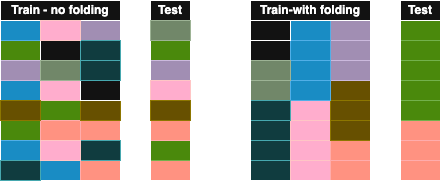
\includegraphics[width=0.8\textwidth]{images/folds.png}
    \caption{Comparison of random train-test splitting and second-level domain (SLD)-based folding. In the diagram, each column represents a fold within the train or test set, each block corresponds to a URL, and each colour represents a distinct second-level domain. It is important that in domain-based folding, the same colour is not in both train and test sets}
    \label{fig:folds}
\end{figure}

When constructing the folds, two constraints should be balanced:
\begin{itemize}
    \item All folds should be approximately equal in size to maintain consistent training and testing set sizes
    \item Each fold should preserve the original class distribution of the dataset (e.g., a 9:1 benign-to-malicious ratio should be maintained within each fold)
\end{itemize}
Table~\ref{tab:sld_folding_statistics} shows an example of how the dataset is distributed when using folding on the Joined dataset.

After initial construction, the folds are sorted by the Gini index of domain frequency, an example of which can be seen in Table~\ref{tab:sld_folding_statistics}. The fold with the lowest Gini index is selected as the test set. This ensures that the test set is as uniform as possible with respect to counts of URLs for SLDs. This helps to avoid scenarios where, for example, a single SLD makes up 12\% of the test set and offers little to helpful none indicators of maliciousness beyond the domain name itself. The model would have no way of detecting these URLs and would be unjustly penalized in such cases, even if it generalizes well. The fact that folds are ordered is also helpful for hyper-parameter tuning because the evaluation set is just picked to be the next fold with the lowest Gini index.

\begin{table}[H]
    \centering
    \renewcommand{\arraystretch}{1.2}
    \resizebox{\textwidth}{!}{
        \begin{tabular}{lllllllllll}
            \toprule
            \textbf{Fold} & \textbf{URLs} & \textbf{SLDs} & \textbf{Benign} & \textbf{Benign \%} & \textbf{Malicious} & \textbf{Malicious \%} & \textbf{Top 1 SLD}    & \textbf{Top 2 SLD} & \textbf{Top 3 SLD}  \\
            \midrule
            0             & 572{,}662     & 245{,}422     & 444{,}298       & 77.58              & 128{,}364          & 22.42                 & geocities (9.3\%)     & appspot (1.8\%)    & alibaba (1.5\%)     \\
            1             & 572{,}351     & 255{,}202     & 449{,}272       & 78.50              & 123{,}079          & 21.50                 & tripod (4.1\%)        & wikipedia (3.1\%)  & blogspot (2.7\%)    \\
            2             & 572{,}349     & 264{,}155     & 444{,}623       & 77.68              & 127{,}726          & 22.32                 & angelfire (3.9\%)     & yahoo (2.5\%)      & imdb (2.3\%)        \\
            3             & 572{,}349     & 274{,}267     & 414{,}583       & 72.44              & 157{,}766          & 27.56                 & 000webhostapp (3.7\%) & ietf (1.1\%)       & sourceforge (0.8\%) \\
            4             & 572{,}349     & 281{,}081     & 442{,}123       & 77.25              & 130{,}226          & 22.75                 & newadvent (2.0\%)     & google (0.6\%)     & about (0.6\%)       \\
            \bottomrule
        \end{tabular}
    }
    \caption{Summary statistics for the 5-fold split of the Joined dataset. Each row corresponds to a fold, showing the number of URLs, number of unique SLDs, class distribution (benign vs. malicious), and the top three most frequent SLDs with their relative frequencies. Fold 4 is used as a test set.}
    \label{tab:sld_folding_statistics}
\end{table}

The effect of domain-aware folding on evaluation performance is shown in Table~\ref{tab:folding_comparison}. Without folding, models appear to perform substantially better in all important metrics. For more information about them, see Section~\ref{sec:metrics}. This is particularly evident in the case of BERT-Tiny~\cite{turc2019} on the private dataset.

A similar case of overestimated performance for smaller models appears when comparing BERT-Small on the GramBeddings dataset in this thesis to the BERT-base results reported in~\cite{domurlbert}. In their work, BERT-base achieved a class 1 F1 score of 0.983 on GramBeddings—the same score obtained here by BERT-Small when domain-aware folding was not applied. This illustrates why results from related work that do not use folding-based evaluation should be interpreted with caution, as they may give an overly optimistic impression of model generalization.

\begin{table}[H]
    \centering
    \renewcommand{\arraystretch}{1.2}
    \resizebox{\textwidth}{!}{
        \begin{tabular}{lllll}
            \toprule
            \textbf{Model} & \textbf{Dataset}                      & \textbf{F1$_1$} & \textbf{Rec$_1$} & \textbf{Prec$_1$} \\
            \midrule
            BERT-Small     & GramBeddings \textbf{Without Folding} & 0.9834          & 0.9820           & 0.9848            \\
            BERT-Small     & GramBeddings With Folding             & 0.9662          & 0.9798           & 0.9530            \\
            \midrule
            BERT-Tiny      & private \textbf{Without Folding}      & 0.935           & 0.9071           & 0.9649            \\
            BERT-Tiny      & private With Folding                  & 0.7565          & 0.6874           & 0.8411            \\
            \bottomrule
        \end{tabular}
    }
    \caption{Comparison of performance with and without SLD-based folding using BERT models with baseline parameters shown in Section~\ref{sec:BERT-Tiny-finetune}. Each model in a pair has the same parameters.}
    \label{tab:folding_comparison}
\end{table}

\section{Exploratory analysis}
This section is based on the \texttt{data\_exploration.ipynb} notebook. The most noteworthy findings were selected and described here.

\subsection{Hostname}

One part of the hostname is TLD. Malicious URLs exhibit distinct TLD distributions compared to benign URLs. Table~\ref{tab:benign_malicious_tld} highlights the differences.

\begin{table}[H]
    \centering
    \renewcommand{\arraystretch}{1.2}
    \resizebox{\textwidth}{!}{
        \begin{tabular}{llllllll}
            \toprule
            \textbf{Dataset} & \textbf{.com (B/M)} & \textbf{.net (B/M)} & \textbf{.org (B/M)} & \textbf{ccTLD (B/M)} & \textbf{Other (B/M)} \\
            \midrule
            GramBeddings     & 49.80\% / 52.52\%   & 3.46\% / 3.77\%     & 8.09\% / 2.97\%     & 26.47\% / 20.39\%    & 11.19\% / 20.34\%    \\
            Kaggle Binary    & 77.06\% / 46.54\%   & 3.32\% / 4.80\%     & 9.68\% / 5.79\%     & 3.94\% / 20.05\%     & 4.04\% / 21.50\%     \\
            Kaggle Multiple  & 72.25\% / 47.12\%   & 4.44\% / 4.86\%     & 8.75\% / 8.22\%     & 7.48\% / 14.70\%     & 5.44\% / 22.40\%     \\
            Mendeley         & 60.98\% / 71.94\%   & 4.58\% / 6.58\%     & 12.33\% / 2.65\%    & 6.22\% / 13.75\%     & 10.60\% / 5.05\%     \\
            Joined           & 61.26\% / 51.33\%   & 4.20\% / 4.28\%     & 11.18\% / 3.97\%    & 9.58\% / 19.94\%     & 9.77\% / 20.01\%     \\
            Private          & 48.48\% / 46.91\%   & 5.73\% / 4.61\%     & 3.23\% / 0.96\%     & 16.52\% / 19.94\%    & 26.02\% / 27.57\%    \\
            \bottomrule
        \end{tabular}
    }
    \caption{Comparison of TLD distributions between benign (B) and malicious (M) URLs. The values were obtained by splitting each dataset into benign and malicious subsets and calculating the percentage of URLs in each subset that contain a given TLD type. CcTLD refers to country-code top-level domains such as \textit{.uk}, \textit{.de}, or \textit{.fr}. The "Other" category includes all remaining TLDs not covered by the standard groups, such as \textit{.xyz}, \textit{.biz}, and .info, as well as URLs that use IP addresses instead of domain names or URLs that contain malformed TLDs.}
    \label{tab:benign_malicious_tld}
\end{table}

Another part of the hostname is SLD. When looking at the datasets, certain second-level domains appear more frequently than others. The information about the content behind the domain is unknown to the model, however, it is useful for the reader to gain insight into what kind of data there are in the dataset.

Many benign URLs belong to widely used platforms like Wikipedia, YouTube, and Facebook. In contrast, malicious URLs frequently originate from free hosting services, dynamic DNS providers, and public cloud platforms.

Malicious SLDs often fall into the following categories:
\begin{itemize}
    \item Free Hosting services: (\textit{000webhostapp}, \textit{netlify}, \textit{appspot}, \textit{pastehtml}) allow easy, anonymous site creation, making them ideal for phishing and malware. Almost all of the URLs containing these SLDs are labelled as malicious.
    \item Free cloud storage services: (\textit{googleapis}, \textit{microsoft}, \textit{google}, \textit{ibm}, \textit{sharepoint}). These can freely host malicious content, making them popular among attackers. It provides valuable insight that just because a URL contains a common serious domain like \textit{google} does not mean it is benign.
    \item Less known SLDs usually have a higher probability of containing malicious intent as they are not yet verified.
\end{itemize}

\subsection{Statistical Analysis of URL Characteristics}
\label{sec:statistical_analysis_url}

To better understand URL structure across datasets, 43 manually engineered features were extracted from the dataset. They were chosen based on the findings from Section~\ref{sec:man_feat_eng}. The code for the features has been from a large majority generated by ChatGPT O1~\cite{openai2025features}. Table~\ref{tab:selected_url_features} shows a subset that highlights key differences by dataset and label. These features are primarily included to give the reader a clearer sense of how the data is distributed. Full statistics are available in the exploration notebook.

Some interesting findings from it are:
\begin{itemize}
    \item Because of pre-filtering for private datasets, many superficial heuristics have reversed values: benign URLs are longer, contain more digits, and have more non-alphanumeric characters than malicious ones.
    \item In datasets like GramBeddings, Joined dataset, and Kaggle Binary, malicious URLs are systematically longer and more complex than benign ones.
    \item The Kaggle Multiple dataset shows that the malware class uses IP-based domains at a much higher rate than the phishing or benign classes, indicating that different attack types exploit different structural patterns.
    \item In public datasets, the presence of an IP address in the URL is a strong indicator of maliciousness, largely because crawlers rarely encounter benign IP-based URLs in the wild. These datasets are biased toward visible web content, where legitimate services typically use domain names. In contrast, the private dataset includes traffic, where IP addresses are also used in benign contexts.
\end{itemize}

\begin{table}[H]
    \centering
    \renewcommand{\arraystretch}{1.2}
    \resizebox{\textwidth}{!}{
        \begin{tabular}{lllllll}
            \toprule
            \textbf{Dataset} & \textbf{Label} & \textbf{URL Length} & \textbf{Num Digits} & \textbf{Non-Alnum} & \textbf{IP in SLD (\%)} & \textbf{kw\_login (\%)} \\
            \midrule
            Private          & Benign         & 186.47              & 38.72               & 17.60              & 6.10                    & 1.75                    \\
            Private          & Malicious      & 121.64              & 18.90               & 12.82              & 5.84                    & 5.43                    \\
            GramBeddings     & Benign         & 46.43               & 1.82                & 8.68               & 0.05                    & 0.54                    \\
            GramBeddings     & Malicious      & 86.21               & 14.98               & 11.83              & 3.36                    & 0.54                    \\
            Joined           & Benign         & 41.01               & 1.33                & 7.95               & 0.04                    & 0.06                    \\
            Joined           & Malicious      & 73.54               & 11.06               & 10.72              & 4.70                    & 0.15                    \\
            Kaggle Binary    & Benign         & 58.30               & 3.26                & 10.46              & 0.09                    & 0.03                    \\
            Kaggle Binary    & Malicious      & 57.80               & 6.01                & 9.33               & 7.52                    & 0.03                    \\
            Kaggle Multiple  & Benign         & 57.69               & 5.60                & 8.51               & 0.14                    & 0.15                    \\
            Kaggle Multiple  & Malware        & 46.55               & 11.07               & 9.40               & 49.90                   & 0.28                    \\
            Kaggle Multiple  & Phishing       & 45.98               & 3.69                & 6.78               & 0.56                    & 0.45                    \\
            Mendeley         & Benign         & 35.84               & 0.79                & 7.22               & 0.03                    & 0.02                    \\
            Mendeley         & Malicious      & 37.20               & 0.29                & 7.68               & 0.00                    & 0.01                    \\
            \bottomrule
        \end{tabular}
    }
    \caption{Key URL statistics by dataset and label. Num Digits counts numeric characters; Non-Alnum counts non-alphanumeric characters; IP in SLD (\%) is the percentage of URLs whose second-level domain is an IP address; kw\_login (\%) is the percentage containing the substring login.}
    \label{tab:selected_url_features}
\end{table}

\subsection{URL Length}
\label{sec:url_length}

The URL length, examined in Table~\ref{tab:url_length_summary}, plays an important role in inference speed, as longer URLs increase the processing time for all model types. In models that rely on batched input, such as BERT, shorter URLs are padded to match the length of the longest sequence in the batch (or the predefined maximum length, whichever is smaller). This padding causes even short URLs to be processed as if they were long, resulting in unnecessary computational overhead. Consequently, measurements on datasets with lower variance in URL length tend to give higher inference speed results. This behaviour is clearly observed on the Mendeley dataset, as discussed in Section~\ref{sec:baselines}. The exact opposite case of that is the private dataset.

\begin{table}[H]
    \centering
    \renewcommand{\arraystretch}{1.2}
    \begin{tabular}{lllll}
        \toprule
        \textbf{Dataset} & \textbf{Mean} & \textbf{Median} & \textbf{Std. Dev.} & \textbf{Max} \\
        \midrule
        GramBeddings     & 66.322        & 49.000          & 59.071             & 7833         \\
        Kaggle Binary    & 58.082        & 49.000          & 39.542             & 2314         \\
        Kaggle Multiple  & 55.191        & 43.000          & 43.944             & 2175         \\
        Mendeley         & 35.872        & 32.000          & 14.440             & 721          \\
        Joined           & 48.593        & 38.000          & 39.577             & 7833         \\
        Private          & 179.990       & 107.000         & 291.134            & 110511       \\
        \bottomrule
    \end{tabular}
    \caption{Summary statistics for raw URL length in each dataset.}
    \label{tab:url_length_summary}
\end{table}

\chapter{Experiments}

This chapter presents the results of all the experiments that were conducted. It begins with an overview of the evaluation metrics used for evaluating all the models. The following section compares several baseline models introduced in the related work chapter~\ref{sec:related_work}, establishing a performance reference for subsequent experiments. The final two sections correspond to the two main approaches outlined in the introduction: designing smaller and faster models that can match the Performance of the baseline and compressing existing models using quantization techniques to increase inference speed.

All experiments were conducted on Databricks Runtime 14.3 ML LTS using a g4dn.xlarge virtual machine with 4 vCPUs, 16~GB of RAM, and an NVIDIA T4 GPU. The libraries used for experiments and their respective versions are detailed in requirements files in the repository. The core ones include PyTorch, Torchvision, Hugging Face Transformers, Scikit-learn, NumPy, Pandas, and MLflow, ONNX Runtime.

In the baseline comparison, all datasets are used, but later experiments focus only on the Private and Joined datasets to reduce computing and avoid issues of individual datasets outlined in Section~\ref{sec:dataset_descriptions}. While one might argue that including all datasets would improve comparability with related work, this is not valid, as prior work does not apply domain-aware folding, which makes direct comparison unreliable.

\section{Metrics}
\label{sec:metrics}
This section first describes the metrics used to evaluate predictive Performance (Table~\ref{tab:metric_formulas}), followed by those used to measure inference speed.

Let $\mathcal{D} = \{(x_i, y_i)\}_{i=1}^{N}$ denote the evaluation set, where $x_i$ is URL, $y_i \in \{0, 1\}$ is the ground truth label, $N$ is the dataset size and $\hat{y}_i$ is the predicted class $c \in C$, where $C$ is set of all available classes. Each model outputs a probability score $s_i \in [0, 1]$ for each class, representing the likelihood that the sample belongs to that class. In multi-class classification, the predicted class is the one with the highest probability: $\hat{y}_i = \arg\max_c s_{i,c}$. In binary classification, predictions are obtained by applying a decision threshold $t$ (unless otherwise specified, the default threshold is $t = 0.5$):

$$
    \hat{y}_i =
    \begin{cases}
        1 & \text{if } s_i \geq t \\
        0 & \text{otherwise}
    \end{cases}
$$


\begin{table}[H]
    \centering
    \renewcommand{\arraystretch}{1.2}
    \setlength{\tabcolsep}{10pt}
    \begin{tabular}{lp{0.7\textwidth}}
        \toprule
        \textbf{Metric}            & \textbf{Formula}                                                                                                        \\
        \midrule
        True Positive (class $c$)  & $\mathrm{TP}_c = \sum_{i}\mathbf{1}\{\hat{y}_i = c \wedge y_i = c\}$                                                    \\
        False Positive (class $c$) & $\mathrm{FP}_{(c)} = \sum_{i}\mathbf{1}\{\hat{y}_i = c \wedge y_i \neq c\}$                                             \\
        False Negative (class $c$) & $\mathrm{FN}_{(c)} = \sum_{i}\mathbf{1}\{\hat{y}_i \neq c \wedge y_i = c\}$                                             \\
        Accuracy                   & $\mathrm{Accuracy} = \frac{1}{N} \sum_{i} \mathbf{1}\{ \hat{y}_i = y_i \}$                                              \\
        Recall (class $c$)         & $\mathrm{Rec}_{(c)} = \mathrm{TP}_{(c)} / (\mathrm{TP}_{(c)} + \mathrm{FN}_{(c)})$                                      \\
        Precision (class $c$)      & $\mathrm{Prec}_{(c)} = \mathrm{TP}_{(c)} / (\mathrm{TP}_{(c)} + \mathrm{FP}_{(c)})$                                     \\
        F1 Score (class $c$)       & $\mathrm{F1}_{(c)} = 2 \cdot \mathrm{Prec}_{(c)} \cdot \mathrm{Rec}_{(c)} / (\mathrm{Prec}_{(c)} + \mathrm{Rec}_{(c)})$ \\
        \midrule
        F1 Score (class $1$)       & $\mathrm{F1}_{(1)} = 2 \cdot \mathrm{Prec}_{(1)} \cdot \mathrm{Rec}_{(1)} / (\mathrm{Prec}_{(1)} + \mathrm{Rec}_{(1)})$ \\
        Recall (class 1)           & $\mathrm{Rec}_{(1)} = \mathrm{TP}_{(1)} / (\mathrm{TP}_{(1)} + \mathrm{FN}_{(1)})$                                      \\
        Precision (class 1)        & $\mathrm{Prec}_{(1)} = \mathrm{TP}_{(1)} / (\mathrm{TP}_{(1)} + \mathrm{FP}_{(1)})$                                     \\
        Macro F1 Score             & $F1_{\text{macro}} = (F1_{(0)} + F1_{(1)}) / 2$                                                                         \\
        ROC AUC                    & Area under ROC curve                                                                                                    \\
        \bottomrule
    \end{tabular}
    \caption{Formulas for evaluation metrics. The upper portion of the table lists auxiliary metrics provided for completeness, while the lower portion includes the primary metrics used in the experiments.}
    \label{tab:metric_formulas}
\end{table}

As described in Section~\ref{sec:real_world_pipeline}. The foremost requirement is to catch as many malicious URLs as possible. The ability of the model to do that is expressed by the recall for the malicious class. Precision for the malicious class is the second critical measure: if it becomes too low, the expensive downstream model is used unnecessarily often. The metric describing how the model balances these two is F1 for the malicious class. Should the F1 score be similar for multiple models, we should prioritize the one with higher recall.

ROC-AUC is another useful metric that provides a threshold-independent evaluation of a model's ability to distinguish between classes. Unlike precision or recall, which depend on a specific decision threshold, ROC-AUC summarizes the trade-off between the true positive rate and false positive rate across all possible thresholds in a ROC curve. The last metric that is shown in comparisons is the macro F1 score.

Additional metrics computed and included in the attached ZIP archive are precision, recall, F1 score, and accuracy for the benign class (class 0), as well as their micro-averaged and weighted variants. Confusion matrices are also provided for all evaluated models.

For each experiment, visualizations of the precision recall and the ROC curves (for class 1) were created to illustrate the model's Performance across different classification thresholds. To keep the attachment file size reasonable, visualizations are included only in selected cases.

When measuring inference speed, there are usually two useful metrics:
\begin{itemize}
    \item \textbf{Throughput (Thr.)} -- the number of items processed per second.
    \item \textbf{Latency (Lat.)} -- the time it takes to process a single input
\end{itemize}

In the context of this thesis, \textbf{throughput} is the more important metric, as the system is expected to handle large quantities of URLs per second, as described in Section~\ref{sec:real_world_pipeline}. Two throughput values are reported in the experiments:
\begin{itemize}
    \item \textbf{Model throughput} -- the number of samples the model alone can process per second, excluding any preprocessing steps. When measuring this metric, it is important to ensure proper synchronization between the GPU and CPUs, as GPU operations are asynchronous by default. Failing to do so may lead to inaccurate or underestimated timing results.
    \item \textbf{Pipeline throughput} -- throughput of the entire inference pipeline, including Tokenization, feature extraction, and model execution. This component is typically easier to scale, as preprocessing steps often run on CPUs, which are more cost-effective to scale out compared to GPUs. Furthermore, using streaming execution, these operations can be overlapped or parallelized so that their computational cost is minimized.
\end{itemize}

The final metric that is reported is the total number of parameters for each model on a given dataset. This thesis defines a parameter as any scalar value the model must store to reconstruct itself for inference (e.g.\ weights, biases, split thresholds, leaf values, etc.).

\section{Baselines}
\label{sec:baselines}
This section presents the Performance of the selected models from the related work chapter, beginning with evaluations on binary classification datasets and concluding with results on multi-class dataset. Additional information about training setup and interesting details for each model are discussed in their respective subsections.

For the feature-based models, Log. Regression, Naive Bayes, and XGBoost were selected. URLNet was chosen as a representative of non-transformer deep learning approaches. For the transformer baseline, BERT-Small~\cite{turc2019}.

\begin{table}[H]
    \resizebox{\textwidth}{!}{
        \begin{tabular}{
            >{\raggedright\arraybackslash}p{3cm}
            lllllllll
            }
            \toprule
            \textbf{Dataset} & \textbf{Model}
                             & \textbf{F1$_1$}
                             & \textbf{Rec$_1$}
                             & \textbf{Prec$_1$}
                             & \textbf{Macro-F1}
                             & \textbf{ROC-AUC}
                             & \textbf{\shortstack{Thr.                                                                          \\Model}}
                             & \textbf{\shortstack{Thr.                                                                          \\Pipeline}}
                             & \textbf{\# params}                                                                                \\
            \midrule

            GramBeddings
                             & Log.\ Regression         & 0.8371 & 0.7789 & 0.9048 & 0.8503 & 0.9151 & 50.4 M  & 19.7 K & 44     \\
                             & Naive Bayes              & 0.7353 & 0.6059 & 0.9349 & 0.7779 & 0.8706 & 1.0 M   & 19.7 K & 88     \\
                             & XGBoost                  & 0.9095 & 0.8784 & 0.9428 & 0.9140 & 0.9700 & 911.8 K & 19.7 K & 6.9 K  \\
                             & URLNet                   & 0.9588 & 0.9304 & 0.9890 & 0.9607 & 0.9944 & 1.2 K   & 893    & 20.8 M \\
                             & BERT-Small               & 0.9662 & 0.9798 & 0.9530 & 0.9664 & 0.9959 & 722     & 641    & 28.8 M \\
            \addlinespace

            Kaggle Binary
                             & Log.\ Regression         & 0.8956 & 0.8373 & 0.9626 & 0.9088 & 0.9399 & 53.6 M  & 21.0 K & 44     \\
                             & Naive Bayes              & 0.4987 & 0.3449 & 0.9001 & 0.6333 & 0.8180 & 1.0 M   & 21.0 K & 88     \\
                             & XGBoost                  & 0.9222 & 0.9032 & 0.9420 & 0.9295 & 0.9754 & 1.0 M   & 21.0 K & 3.8 K  \\
                             & URLNet                   & 0.9971 & 0.9957 & 0.9985 & 0.9973 & 0.9998 & 1.2 K   & 894    & 15.6 M \\
                             & BERT-Small               & 0.9973 & 0.9955 & 0.9992 & 0.9976 & 0.9999 & 963     & 845    & 28.8 M \\
            \addlinespace

            Mendeley
                             & Log.\ Regression         & 0.0912 & 0.5174 & 0.0500 & 0.4763 & 0.6981 & 55.3 M  & 25.0 K & 44     \\
                             & Naive Bayes              & 0.0505 & 0.9647 & 0.0260 & 0.1440 & 0.6763 & 1.0 M   & 25.0 K & 88     \\
                             & XGBoost                  & 0.1507 & 0.3738 & 0.0944 & 0.5493 & 0.7387 & 501.3 K & 25.0 K & 41.7 K \\
                             & URLNet                   & 0.6475 & 0.4896 & 0.9557 & 0.8206 & 0.9376 & 1.2 K   & 979    & 32.3 M \\
                             & BERT-Small               & 0.6980 & 0.5911 & 0.8522 & 0.8460 & 0.9550 & 3.1 K   & 2.6 K  & 28.8 M \\
            \addlinespace

            Joined
                             & Log.\ Regression         & 0.7103 & 0.7996 & 0.6389 & 0.8053 & 0.8991 & 60.7 M  & 20.0 K & 44     \\
                             & Naive Bayes              & 0.5993 & 0.4771 & 0.8055 & 0.7553 & 0.8346 & 923.5 K & 20.0 K & 88     \\
                             & XGBoost                  & 0.8223 & 0.8406 & 0.8047 & 0.8842 & 0.9488 & 657.3 K & 20.0 K & 18.5 K \\
                             & URLNet                   & 0.8969 & 0.8321 & 0.9727 & 0.9347 & 0.9786 & 1.6 K   & 982    & 57.9 M \\
                             & BERT-Small               & 0.9322 & 0.9149 & 0.9501 & 0.9563 & 0.9845 & 731     & 645    & 28.8 M \\
            \addlinespace

            Private Data
                             & Log.\ Regression         & 0.3677 & 0.7833 & 0.2402 & 0.6073 & 0.8175 & 48.2 M  & 16.8 K & 44     \\
                             & Naive Bayes              & 0.1927 & 0.8452 & 0.1087 & 0.3261 & 0.7392 & 901.4 K & 16.8 K & 88     \\
                             & XGBoost                  & 0.5883 & 0.7891 & 0.4689 & 0.7653 & 0.9226 & 488.4 K & 16.8 K & 9.2 K  \\
                             & URLNet                   & 0.7555 & 0.6248 & 0.9555 & 0.8678 & 0.9538 & 1.6 K   & 794    & 59.7 M \\
                             & BERT-Small               & 0.8648 & 0.8103 & 0.9271 & 0.9261 & 0.9599 & 497     & 429    & 28.8 M \\
            \bottomrule
        \end{tabular}
    }
    \caption{Performance, throughput, and parameter counts of classification models across five binary datasets that use domain-aware folding.}
    \label{tab:baseline_binary_classification_results}
\end{table}

Table~\ref {tab:baseline_binary_classification_results} presents a performance summary of the selected baseline models. In terms of $\mathrm{F}1_1$, BERT-Small consistently performs best. URLNet is next, followed by XGBoost and Log. Regression and Naive Bayes. While URLNet typically achieves higher $\mathrm{Prec}_1$ than BERT-Small, its $\mathrm{Rec}_1$, which is a more important metric to maximize (as described in the metrics Section~\ref{sec:metrics}), is worse. Some feature-based models like Naive Bayes seem to have higher $\mathrm{Rec}_1$ than BERT-Small, especially on imbalanced datasets. Still, they struggle with $\mathrm{Prec}_1$, severely limiting their practical usefulness.

As far as datasets are concerned, Kaggle Binary is the easiest. It is balanced and consists of easily separable examples, as the near-perfect Performance suggests across multiple models. GramBeddings dataset, while also balanced, is slightly more challenging but still solvable with high scores. Mendeley dataset seems to be the hardest, because of the severe imbalance and lower amount of malicious samples compared to other datasets.

The throughput for the feature-based models is significantly higher for all datasets. However, this is kept down by the necessity of creating features from URL, which bottlenecks these models significantly. For deep learning models, the throughput is much lower and is heavily dependent on the data. For example, Mendeley contains very similar length URLs that are very short, as discussed in~\ref{sec:url_length}, so BERT-Small is significantly faster there. The exact opposite is true for the private datasets, where URLs vary in size a lot, and URLNet, which uses more aggressive truncation, has the upper hand over BERT-Small even though it has more parameters.

\subsection{Feature based models}
\label{sec:feature_models}

These models use the same 43 handcrafted features extracted from the URL that were described in Section~\ref{sec:statistical_analysis_url}. For hyper-parameter tuning, the original training set was further divided into training and validation subsets. Specifically, the last fold was reserved as the validation set. This results in a 60/20/20 split (training/validation/test) for the public datasets and an 80/10/10 split for the private dataset. For Log. regression, StandardScalar was applied. It is a preprocessing technique that standardizes each feature. The scaler was fitted on the training set and then applied to the Evaluation set to ensure consistent feature scaling. All of the models were evaluated on CPU.

Hyper-parameters for all models were optimized using randomized grid search. All configuration details and best parameters are recorded in the same notebook. No oversampling, under-sampling, or class weighting was applied to the data directly. Instead, Log. Regression and XGBoost were given class ratio parameters, which should alter their training process to consider the imbalance.

Feature importance was computed for both Log. Regression and XGBoost across all datasets. Identifying which features are truly predictive is useful, as the current inference performance on the private dataset plateaus at around 16,788 samples per second when using all 43 features. Removing less relevant features could improve speed. Additionally, the results provide insight into which types of information are present and useful in each dataset.

\begin{itemize}
    \item \textbf{Private dataset:} Presence of the \texttt{@} character, number of subdomains, number of question marks in the URL, total length of the query string, and number of path segments in the URL path.

    \item \textbf{Joined dataset:} Presence of the keyword \texttt{login}, use of a suspicious top-level domain (TLD), number of subdomains, presence of the keyword \texttt{secure}, and presence of the keyword \texttt{update}.
\end{itemize}

The code for training these models is provided in the notebook \wrappedttt{feature\_models.ipynb}

\subsection{URLNet}
This model, described in Section~\ref{sec:dl_models}, was chosen to represent non-transformer deep learning approaches. According to related work~\cite{TransURL}, transformer-based models consistently outperform traditional deep learning methods on URL classification tasks. Therefore, only a single representative from this category was included.

URLNet was trained and evaluated on a GPU. The model uses both character-level and word-level convolutional branches, corresponding to embedding mode 5. All other hyper-parameters were kept at their default values as defined in the original codebase.

Originally, URLNet was implemented in TensorFlow 1.8, which is not supported on the Databricks platform. To address this, the necessary parts of the code were adapted for TensorFlow 2.14, and the resulting code has been stored in the \texttt{baselines/URLNet} directory. The entire training and evaluation pipeline can be executed using the \wrappedttt{baseline\_run\_urlnet.ipynb} notebook.

It can be observed, that the model has very different number of parameters based on what dataset it is being trained on. This is because the total parameter count includes also the embedding matrices, which depend on the vocabulary sizes. Since each dataset produces a different character and word vocabulary (based on token frequency thresholds), the resulting embedding layers differ in size.

\subsection{BERT-Small}
\label{baseline:bert_small}
The model architecture and default hyper-parameters are based on the pre-trained Hugging Face model \texttt{google/bert\_uncased\_L-4\_H-512\_A-8},\footnote{\nolinkurl{https://huggingface.co/google/bert_uncased_L-4_H-512_A-4}} which provides a smaller and faster alternative to standard BERT models. Since the goal of the thesis is to increase throughput, other experiments do not use BERT variants larger than BERT-Small.

The following list describes hyper-parameters used for training the model that were used for training the baseline model provided by the supervisor:
\begin{itemize}
    \item \textbf{Architectural parameters} -- These are the default parameters from the Hugging Face model. \#encoder layers = 4, hidden size = 512, \#attention heads = 8, intermediate size = 2048, activation = GELU, dropout = 0.1 (hidden and attention), max position embeddings = 512, vocabulary size = 30,522, positional encoding=absolute, LayerNorm $\epsilon$=10e-12.

    \item \textbf{Training} -- Maximum sequence length = 256, batch size = 128, \#train epochs = 2, loss = Focal~\cite{lin2018focallossdenseobject} ($\gamma=2$, $\alpha=\mathrm{Not used}$), LR = 10e-5 for entire model, weight decay = 0, optimizer = AdamW.

    \item \textbf{Tokenization} -- Hugging Face AutoTokenizer with padding and truncation enabled, maximum sequence length before truncation = 256.
\end{itemize}

\subsection{Multi-class classification}
\label{sec:multi_class_experiment}
This section evaluates the baseline models on the Kaggle Multiple dataset to assess whether multi-class classification remains effective when domain-aware folding is applied. That is a scenario not previously explored in related work. The Kaggle Multiple dataset is very similar to the Kaggle Binary dataset, which is known to be easy to train on, as shown in Table~\ref{tab:baseline_binary_classification_results}. For this reason, and because multi-class labels are not available for the private dataset that reflects real-world conditions, the multi-class Evaluation is included only in this section. All subsequent experiments focus solely on binary classification.

The main metrics that should be examined in this case are individual F1 scores on malicious classes and also macro F1 score. Table~\ref{tab:multiclass_kaggle_multiple} presents the results. The BERT-Small model differentiates between classes with high consistency, achieving an F1 scores above 0.9 for all classes and macro. This confirms that transformer-based models could effectively generalize across multiple malicious categories, even when relying solely on URL strings, although confirming this would require Evaluation of real-world data.

URLNet is not included in these multi-class benchmarks, as its original implementation supports only binary classification and extending it for multi-class scenarios would require substantial code modifications to the URLNet training script not justified for a baseline-only evaluation.

\begin{table}[H]
    \centering
    \resizebox{\textwidth}{!}{
        \begin{tabular}{
            >{\raggedright\arraybackslash}p{3cm}
            llllllll
            }
            \toprule
            \textbf{Model}
                            & \textbf{Malware-F1}
                            & \textbf{Phishing-F1}
                            & \textbf{Macro-F1}
                            & \textbf{Macro-Prec.}
                            & \textbf{Macro-Rec.}
                            & \textbf{\shortstack{Thr.                                                                 \\Model}}
                            & \textbf{\shortstack{Thr.                                                                 \\Pipeline}}
                            & \textbf{\# Params}                                                                       \\
            \midrule
            Log. Regression & 0.7137                   & 0.4946 & 0.6696 & 0.6429 & 0.7694 & 27.1 M  & 20.1 K & 132    \\
            Naive Bayes     & 0.1627                   & 0.2367 & 0.3548 & 0.4389 & 0.5089 & 931.1 K & 20.1 K & 132    \\
            XGBoost         & 0.7932                   & 0.7715 & 0.8398 & 0.8850 & 0.8139 & 516.5 K & 20.1 K & 16.7 K \\
            BERT-Small      & 0.9244                   & 0.9093 & 0.9379 & 0.9459 & 0.9319 & 604     & 539    & 28.8 M \\
            \bottomrule
        \end{tabular}
    }
    \caption{Multi-class classification performance of selected models on the Kaggle Multiple dataset.}
    \label{tab:multiclass_kaggle_multiple}
\end{table}

\section{Training faster models}

The first approach to improving the trade-off between throughput and predictive Performance is to start with a smaller, faster model and enhance its accuracy to approach that of the baselines. Table~\ref{tab:bert_model_selection} compares different BERT-Tiny and BERT-Mini variants from~\cite{turc2019} in terms of speed and baseline performance. This section focuses on that through the following steps:
\begin{itemize}
    \item Conducting an ablation study on BERT-Tiny hyper-parameters to identify changes that could lead to performance improvements.
    \item Introducing a novel data augmentation method -— domain masking.
\end{itemize}
Finally, both model variants are trained on the full training set from the joined and private datasets using the insights and methods described above.

\begin{table}[H]
    \centering
    \resizebox{\textwidth}{!}{
        \begin{tabular}{lllllllllccc}
            \toprule
            \textbf{Model}
                       & \textbf{F1$_1$}
                       & \textbf{Rec$_1$}
                       & \textbf{Prec$_1$}
                       & \textbf{Macro-F1}
                       & \textbf{ROC-AUC}
                       & \textbf{\shortstack{Thr.                                                                                 \\Model}}
                       & \textbf{\shortstack{Thr.                                                                                 \\Pipeline}}
                       & \textbf{\#Params}
                       & \textbf{\shortstack{Encoder                                                                              \\Layers}}
                       & \textbf{\shortstack{Hidden                                                                               \\size}}
                       & \textbf{\shortstack{Attention                                                                            \\Heads}}                               \\
            \midrule
            BERT-Tiny  & 0.7565                        & 0.6874 & 0.8411 & 0.8672 & 0.9443 & 4,939 & 1,917 & 4.4 M  & 2 & 128 & 2 \\
            BERT-Mini  & 0.8166                        & 0.7365 & 0.9162 & 0.9001 & 0.9548 & 1,528 & 1,008 & 11.2 M & 4 & 256 & 4 \\
            BERT-Small & 0.8648                        & 0.8103 & 0.9271 & 0.9261 & 0.9599 & 497   & 429   & 28.8 M & 4 & 512 & 8 \\
            \bottomrule
        \end{tabular}
    }
    \caption{Comparison of BERT-Tiny, BERT-Mini, and BERT-Small on the private test set. Each model was trained on the full training set. Throughput is measured both for the model forward pass and for the full pipeline, including Tokenization.}
    \label{tab:bert_model_selection}
\end{table}

\subsection{BERT-Tiny ablation study}
\label{sec:BERT-Tiny-finetune}
A specific set of hyper-parameters was chosen as the ablation baseline, denoted as A0, and in each run, one or more parameters of A0 were modified. The resulting Performance was then compared to A0 to assess the Impact of each parameter value. The ablation study is done both on private and public dataset. It is crucial to perform the studies on a validation set rather than the test set, as the results directly inform the selection of hyper-parameters for subsequent models.

A0 is derived from the baseline configuration described in Section~\ref{baseline:bert_small}, denoted as B0. Several new hyper-parameters were added or changed. Since A0 outperformed B0 in terms of predictive Performance on both private and joined datasets, it was selected as the starting point for the ablation study instead of B0. The key changes are summarized below:

\begin{itemize}
    \item Train epochs = 5
    \item Hidden dropout = 0 to increase the capacity of the BERT-Tiny model, which is already highly constrained.
    \item Add weight decay = 0.01 to compensate for the decrease in dropout.
    \item Freeze BERT encoder for the first epoch of training, allowing only the randomly initialized classifier head to be updated. This aims to stabilize training and reduce the risk of catastrophic forgetting in such a small model.
    \item Separate learning rates were used for the encoder and classifier: LR$_{\text{BERT}}$ = 3e-5 and LR$_{\text{clf}}$ = 2e-3, to address the different initialization states of the two components.
\end{itemize}

\subsubsection*{Ablation on private data}
\label{sec:private_ablation}
The dataset was initially split into 80\% training, 10\% validation, and 10\% test. One fold (1/9 of the training portion) was held out as a validation set, and the remaining eight folds were used for training. 30\% of each training fold was used and selected through stratified sampling to preserve class balance. Despite this down-sampling, the resulting training remained large (683,608 training samples and 297,071 validation samples). Since only relative comparison is important here, this approach should be valid way to select hyper-parameters.

Table~\ref{tab:bert_tiny_ablation} presents the full ablation study. Changes that increase $F1_1$ or do not change it significantly and increase Rec$_1$ are labelled with the U prefix (U1, ...) and changes which decrease it have a D prefixed label.

\begin{table}[H]
    \centering
    \resizebox{\textwidth}{!}{
        \begin{tabular}{llllllll}
            \toprule
            ID & Modified factor(s)               & \textbf{F1$_1$} & \textbf{Rec$_1$} & \textbf{Prec$_1$} & \textbf{Macro-F1} & \textbf{ROC-AUC} & \textbf{Best epoch} \\
            \midrule
            B0 & Baseline (max 2 epochs)          & 0.553           & 0.413            & 0.837             & 0.776             & 0.909            & 1                   \\
            B1 & Baseline (max 5 epochs)          & 0.590           & 0.439            & 0.898             & 0.776             & 0.896            & 4                   \\
            A0 & Ablation baseline                & 0.622           & 0.484            & 0.870             & 0.793             & 0.915            & 2                   \\
            \midrule
            U1 & Focal $\alpha=0.7$               & \textbf{0.740}  & \textbf{0.653}   & 0.853             & 0.855             & 0.933            & 2                   \\
            U2 & Unfreeze BERT from start         & 0.698           & 0.579            & 0.880             & 0.833             & 0.903            & 3                   \\
            U3 & Dropout = 0.1                    & 0.676           & 0.541            & 0.902             & 0.822             & 0.931            & 2                   \\
            U4 & Lower learning rates (both 1e-5) & 0.655           & 0.513            & 0.904             & 0.811             & 0.914            & 5                   \\
            U5 & Weight decay = 0                 & 0.620           & 0.521            & 0.765             & 0.790             & 0.891            & 4                   \\
            \midrule
            D1 & Max sequence length = 128        & 0.614           & 0.457            & 0.939             & 0.789             & 0.914            & 2                   \\
            D2 & Focal $\gamma=1$                 & 0.595           & 0.441            & 0.912             & 0.779             & 0.899            & 3                   \\
            \bottomrule
        \end{tabular}
    }
    \caption{Ablation study of BERT-Tiny on the private dataset}
    \label{tab:bert_tiny_ablation}
\end{table}

Multiple observations can be made about the table.
\begin{itemize}
    \item U1: Using Focal loss with $\alpha = 0.7$ increases both $F1_1$ and Rec$_1$. The $\alpha$ parameter acts as a class weighting term that emphasizes the minority class, which encourages the model to focus on classifying them correctly. This is especially useful in this scenario because of the dataset imbalance and the fact that Rec$_1$ is important.
    \item U2: Contrary to expectations, freezing the BERT layers at the start of training did not lead to performance improvements.
    \item U3: Removing dropout did not actually help. Therefore, future values will be set to the default value of the models.
    \item U4: Decreasing learning rate seems to increase Performance when combined with frozen BERT layers in the first epoch.
    \item U5: Weight decay seems to have a negative impact on recall. Therefore, it will not be used.
    \item D1: Reducing the maximum sequence length to 128 harms performance slightly. It indicates that valuable information is being discarded.
    \item D2: Lowering $\gamma$ from 2 to 1 weakens the ability of the focal loss to focus more on hard examples instead of the easy ones as described in. This mechanism is in detail explored in~\cite{lin2018focallossdenseobject}
\end{itemize}

Based on the ablation results, the final model configurations are derived by applying the parameter changes marked with a U prefix to the A0 setup. Let this parameter combination be denoted as \textit{Abl Priv.}. Focal loss is used with $\gamma = 2$ and $\alpha = 0.7$, weight decay is set to 0, and the hidden dropout rate is 0.1. The BERT encoder is unfrozen from the start, and a learning rate of 1e-5 is applied uniformly. The maximum sequence length is 256. The number of training epochs is set to 4, as only one model showed improvement beyond that point.

Even though this process does not guarantee an optimal parameter combination, since it does not account for potential interactions between parameters, serves as useful heuristic for finding improved configurations.

\subsubsection*{Ablation on Joined dataset}
\label{sec:BERT-Tiny-finetune-joined}
A similar experiment was conducted on the Joined dataset, using the same ablation baseline A0. For this experiment, 60\% of the dataset was allocated for training and 20\% for validation. The remaining 20\% was reserved for the test set, which remained untouched throughout the study.

Interestingly, the baseline ablation model (A0) turned out to be the best-performing configuration in this setting. It highlights how misleading the public datasets can be, and if hyper-parameters are tuned solely on them, the resulting models may not generalize well to real-world data.

\begin{table}[H]
    \centering
    \resizebox{\textwidth}{!}{
        \begin{tabular}{llllllll}
            \toprule
            ID & Modified factor(s)               & \textbf{F1$_1$} & \textbf{Rec$_1$} & \textbf{Prec$_1$} & \textbf{Macro-F1} & \textbf{ROC-AUC} & \textbf{Best epoch} \\
            \midrule
            B0 & Baseline                         & 0.932           & 0.907            & 0.959             & 0.954             & 0.988            & 5                   \\
            A0 & Ablation baseline                & \textbf{0.942}  & \textbf{0.922}   & \textbf{0.963}    & \textbf{0.960}    & \textbf{0.989}   & \textbf{4}          \\
            \midrule
            D1 & Dropout = 0.1                    & 0.941           & 0.924            & 0.959             & 0.960             & 0.990            & 5                   \\
            D2 & Classifier learning rate = 0.005 & 0.941           & 0.916            & 0.966             & 0.959             & 0.988            & 5                   \\
            D3 & Unfreeze BERT from start         & 0.941           & 0.920            & 0.963             & 0.959             & 0.988            & 4                   \\
            D4 & Focal $\gamma=1$                 & 0.940           & 0.921            & 0.961             & 0.959             & 0.988            & 5                   \\
            D5 & Weight decay = 0                 & 0.940           & 0.921            & 0.959             & 0.959             & 0.989            & 5                   \\
            D6 & Focal $\alpha=0.7$               & 0.938           & 0.922            & 0.954             & 0.957             & 0.989            & 3                   \\
            D7 & BERT learning rate = 1e-5        & 0.932           & 0.910            & 0.956             & 0.954             & 0.986            & 4                   \\
            D8 & Max sequence length = 128        & 0.929           & 0.908            & 0.950             & 0.951             & 0.987            & 2                   \\
            D9 & Keep BERT layers frozen          & 0.721           & 0.631            & 0.841             & 0.816             & 0.922            & 2                   \\
            \bottomrule
        \end{tabular}
    }
    \caption{Ablation study of BERT-Tiny on the joined dataset}
    \label{tab:bert_tiny_joined_ablation}
\end{table}

\subsection{Domain masking}
\label{sec:domain_masking}
Section~\ref{sec:train_test_split} discusses the necessity of using domain-aware folding during Evaluation but does not address how to prevent the model from memorizing domains during training. This is crucial, as approximately 98\% of second-level domains are associated exclusively with either benign or malicious URLs, making it easy for the model to achieve near-perfect Performance on the training set through memorization.

To mitigate this issue, a novel augmentation technique is proposed. The method works as follows:

\begin{itemize}
    \item During batch construction, for each URL, a paired version is created in which the second-level domain is replaced with the special \texttt{[MASK]} substring. The \texttt{[MASK]} token is already part of the tokenizer vocabulary, which means that the result of Tokenization will be one token.
    \item All examples (original and masked) are shuffled to avoid having paired examples in consecutive order, which could otherwise allow the model to pick up positional correlations.
    \item For URLs that do not contain a second-level domain, a paired masked version is still created to ensure uniform treatment and avoid de-prioritizing those samples.
\end{itemize}

This augmentation strategy forces the model to rely on other types of information at every step of the training. If the domain is the only information that can be used to identify the sample, the model can still learn to rely on it. This ensures that such examples do not increase training loss or destabilize training.

The underlying intuition is that this approach should improve generalization for models of all sizes but is likely to be particularly beneficial for BERT-Mini or BERT-Small. This is because the method encourages the model to learn both domain-related and domain-independent features, and smaller models may not have sufficient capacity to effectively capture both. For this reason, only BERT-Mini will be trained using domain masking.

Since the number of URLs effectively doubles, it is practical to reduce the number of training epochs by half to maintain a consistent training duration.
\subsection{Training BERT-Tiny, BERT-Mini}

Table~\ref{tab:private_train} presents a comparison of baseline models to the fine-tuned BERT-Tiny and BERT-Mini variants on the private dataset. Among the fine-tuned models, the domain-masked BERT-Mini stands out as the best. It achieves the highest Rec$_1$ and comes very close to the BERT-Small baseline in terms of F1$_1$, making it the best overall model for this task—especially considering that high recall is the primary objective. Notably, even the standard BERT-Mini model (without domain masking) surpasses BERT-Small in recall. In contrast, BERT-Tiny does not reach a sufficient level of Performance, suggesting that its capacity is insufficient for the task, even when fine-tuned.

\begin{table}[H]
    \centering
    \resizebox{\textwidth}{!}{
        \begin{tabular}{llllllll}
            \toprule
            \textbf{Model}          & \textbf{F1$_1$} & \textbf{Rec$_1$} & \textbf{Prec$_1$} & \textbf{Macro-F1} & \textbf{ROC-AUC} \\
            \midrule
            BERT-Tiny (B0)          & 0.7565          & 0.6874           & 0.8411            & 0.8672            & 0.9443           \\
            BERT-Mini  (B0)         & 0.8166          & 0.7365           & 0.9162            & 0.9001            & 0.9548           \\
            BERT-Small  (B0)        & \textbf{0.8648} & 0.8103           & 0.9271            & 0.9261            & 0.9599           \\
            \midrule
            BERT-Tiny  (Abl Priv.)  & 0.7747          & 0.7290           & 0.8265            & 0.8767            & 0.9383           \\
            BERT-Mini  (Abl Priv.)  & 0.8248          & 0.8312           & 0.8185            & 0.9035            & 0.9632           \\
            \textbf{BERT-Mini (DM)} & \textbf{0.8625} & \textbf{0.8368}  & \textbf{0.8899}   & \textbf{0.9246}   & 0.9589           \\
            \bottomrule
        \end{tabular}
    }
    \caption{Results on the private dataset. All models listed in the lower section were trained using hyper-parameters derived from an ablation study conducted on the private dataset (Abl Priv.). The domain-masked BERT-mini (DM) was also trained using Abl. Priv. parameters, but only two epochs, as the number of training samples effectively doubled.}
    \label{tab:private_train}
\end{table}

A similar comparison is performed on the joined dataset. For this case, BERT-Tiny with the A0 configuration is used, as it achieved the best results on the dataset. The BERT-Mini models, however, are trained using the (Abl Priv.) configuration. This is because the best hyper-parameter configuration can be seen in Table~\ref{tab:bert_tiny_joined_ablation} for BERT-Tiny may not generalize to BERT-Mini, but the insights from individual ablations remain applicable across model sizes.

Once again, the domain-masked BERT-Mini outperforms the others~\ref{tab:joined_train_results}, achieving the highest Rec$_1$ and a comparable F1$_1$ to the remaining models. Notably, if the Evaluation were limited to public datasets, the results might misleadingly suggest that BERT-Tiny performs well. However, as shown in the previous table, this does not hold true in real-world data.

\begin{table}[H]
    \centering
    \resizebox{\textwidth}{!}{
        \begin{tabular}{llllllll}
            \toprule
            \textbf{Model}                               & \textbf{F1$_1$} & \textbf{Rec$_1$} & \textbf{Prec$_1$} & \textbf{Macro-F1} & \textbf{ROC-AUC} \\
            \midrule
            BERT-Small (B0)                              & 0.9322          & 0.9149           & 0.9501            & 0.9563            & 0.9845           \\
            \midrule
            BERT-Tiny  (A0)                              & 0.9220          & 0.8941           & 0.9516            & 0.9499            & 0.9812           \\
            BERT-Mini  (Abl Priv.)                       & 0.9327          & 0.9132           & 0.9530            & 0.9567            & 0.9872           \\
            \textbf{BERT-Mini domain masked} (Abl Priv.) & 0.9293          & \textbf{0.9210}  & 0.9378            & 0.9544            & 0.9875           \\
            \bottomrule
        \end{tabular}
    }
    \caption{Results on the joined dataset}
    \label{tab:joined_train_results}
\end{table}

This section shows that BERT-Mini with domain masking can serve as a viable substitute for BERT-Small, offering similar or improved predictive Performance while achieving three times higher model throughput, as shown in Table~\ref{tab:bert_model_selection}.

\section{Model Compression and Acceleration}
This section presents the experimental results of the compression techniques outlined in Section~\ref{sec:model_compression_methods}, applied to the BERT-Small with baseline parameters and the domain-masked BERT-Mini models on both the private and joined datasets. First, static quantization is discussed in detail. Subsequently, experiments with dynamic quantization are described. Finally, a comparison of all methods enabling GPU execution is provided and evaluated on the complete test set for both datasets and models.

\subsection{Static quantization}
\label{sec:static_quant_experiments}

For static quantization, the Transformer Deploy library~\cite{els-rd_transformer-deploy_2025} was used. The default set of operations provided by the library was selected for the experiments, while all remaining operations were kept in \wrappedttt{Float32}. The following operations were quantized to \wrappedttt{Int8}: Matrix multiplications (MatMul), Element-wise additions (Add), Batched matrix multiplications (BMM), Layer normalization (LayerNorm), Linear (fully connected) layers.

The actual quantization is performed by inserting fake quantization and dequantization nodes into the PyTorch model, which are then exported to ONNX. At runtime, these nodes are used to build an actual quantized model using NVIDIA TensorRT execution provider \footnote{More information about can be found in: \nolinkurl{https://docs.nvidia.com/deeplearning/tensorrt/latest/getting-started/quick-start-guide.html}}. Evaluation has been done on both the built TensorRT variants and PyTorch fake-quantized version and they match in terms of predictive Performance.

The experiments use percentile calibration with a 99.9\% coefficient with 1000 calibration samples from the training dataset. Several other coefficients were tested on the validation dataset using the BERT-small model with B0 parameters. Table~\ref{tab:static_quant_percentiles} summarizes the results. Even though the F1$_1$ is the lowest for 99.9, Rec$_1$ is the highest, which makes it suitable for the task.

\begin{table}[H]
    \centering
    \resizebox{\textwidth}{!}{
        \begin{tabular}{llllll}
            \toprule
            \textbf{Percentile} & \textbf{F1$_1$} & \textbf{Rec$_1$} & \textbf{Prec$_1$} & \textbf{Macro-F1} & \textbf{ROC-AUC} \\
            \midrule
            99.9                & 0.8620          & 0.8187           & 0.9100            & 0.9244            & 0.9542           \\
            99.99               & 0.8640          & 0.8110           & 0.9243            & 0.9256            & 0.9555           \\
            99.999              & 0.8693          & 0.8102           & 0.9377            & 0.9286            & 0.9562           \\
            99.9999             & 0.8648          & 0.8031           & 0.9368            & 0.9262            & 0.9556           \\
            \bottomrule
        \end{tabular}
    }
    \caption{Impact of calibration percentile on validation performance (BERT-small)}
    \label{tab:static_quant_percentiles}
\end{table}

The \wrappedttt{quantization\_end\_to\_end} from~\cite{els-rd_transformer-deploy_2025} was used as a starting point for the code in the thesis. However, the provided example notebooks could not be reproduced, probably due to version incompatibilities. As a result, modifications to the library were made and stored in the \wrappedttt{libraries} folder. These adjustments were made with the assistance of the O1 ChatGPT model.

For reproducibility purposes, the TensorRT builder requires sufficient workspace size. For the BERT-small model, a workspace of 4 GB is necessary, while 1 GB suffices for the BERT-mini variant. Insufficient workspace allocation prevents the model from being built.

\subsection{Dynamic quantization}
\label{sec:dynamic_quant_experiments}

Dynamic quantization was performed using ONNX Runtime and evaluated on a limited subset of 16,000 samples from the test set of each dataset, as GPU execution is not supported. The configuration applied 8-bit integer quantization to weights, targeted MatMul and Gemm (General matrix multiply) operations, enabled per-channel quantization.

\begin{table}[H]
    \centering
    \resizebox{\textwidth}{!}{
        \begin{tabular}{
            >{\raggedright\arraybackslash}p{1.2cm}
            >{\raggedright\arraybackslash}p{3.3cm}
            llllll
            }
            \toprule
            \textbf{Dataset}
             & \textbf{Model}
             & \textbf{Compression method}
             & \textbf{F1$_1$}
             & \textbf{Rec$_1$}
             & \textbf{Prec$_1$}
             & \textbf{Thr. Model}
             & \textbf{Thr. Pipeline}                                                                                    \\
            \midrule
            Private
             & BERT-Mini (DM)              & Dynamic quantization & 0.8495 & 0.8373 & 0.8621 & 85  (1.42x) & 82  (1.41x) \\
             &                             & CPU baseline         & 0.8515 & 0.8325 & 0.8712 & 60  (1.00x) & 58  (1.00x) \\
             & BERT-Small (B0)             & Dynamic quantization & 0.8647 & 0.7908 & 0.9538 & 24  (1.19x) & 24  (1.19x) \\
             &                             & CPU baseline         & 0.8619 & 0.7997 & 0.9345 & 20  (1.00x) & 20  (1.00x) \\
            Joined
             & BERT-Mini (DM)              & Dynamic quantization & 0.9280 & 0.9154 & 0.9410 & 198 (1.48x) & 191 (1.46x) \\
             &                             & CPU baseline         & 0.9289 & 0.9184 & 0.9396 & 134 (1.00x) & 131 (1.00x) \\
             & BERT-Small (B0)             & Dynamic quantization & 0.9278 & 0.9126 & 0.9435 & 65  (2.62x) & 64  (2.60x) \\
             &                             & CPU baseline         & 0.9289 & 0.9118 & 0.9467 & 25  (1.00x) & 25  (1.00x) \\
            \bottomrule
        \end{tabular}
    }
    \caption{Performance and throughput of dynamically quantized BERT models on the limited subset of test part joined and private datasets on CPU.}
    \label{tab:dynamic_quant_summary}
\end{table}

\subsection{Results discussion}
\begin{table}[H]
    \centering
    \resizebox{\textwidth}{!}{
        \begin{tabular}{
            >{\raggedright\arraybackslash}p{1.2cm}
            >{\raggedright\arraybackslash}p{3.3cm}
            llllll
            }
            \toprule
            \textbf{Dataset}
             & \textbf{Model}
             & \textbf{Compression method}
             & \textbf{F1$_1$}
             & \textbf{Rec$_1$}
             & \textbf{Prec$_1$}
             & \textbf{Thr. Model}
             & \textbf{Thr. Pipeline}                                                                                                                    \\
            \midrule
            \addlinespace
            Private
             & BERT-Mini (DM)              & Float16 optimized     & 0.8625 & 0.8367          & 0.8899 & \textbf{4,705 (2.94x)} & \textbf{1,701 (1.62x)} \\
             &                             & Static quant.         & 0.8408 & \textbf{0.8461} & 0.8355 & 3,688 (2.31x)          & 1,530 (1.46x)          \\
             &                             & Quant. aware training & 0.8534 & 0.8149          & 0.8956 & 3,688 (2.31x)          & 1,530 (1.46x)          \\
             &                             & Optimized baseline    & 0.8625 & 0.8368          & 0.8899 & 2,015 (1.26x)          & 1,206 (1.15x)          \\
             &                             & GPU baseline          & 0.8625 & 0.8368          & 0.8899 & 1,598 (1.00x)          & 1,049 (1.00x)          \\
             & BERT-Small (B0)             & Float16 optimized     & 0.8649 & 0.8104          & 0.9272 & 3,166 (6.43x)          & 1,573 (3.68x)          \\
             &                             & Static quant.         & 0.8595 & 0.8168          & 0.9069 & 2,335 (4.74x)          & 1,357 (3.18x)          \\
             &                             & Quant. aware training & 0.8486 & 0.7800          & 0.9304 & 2,335 (4.74x)          & 1,357 (3.18x)          \\
             &                             & Optimized baseline    & 0.8648 & 0.8103          & 0.9271 & 545 (1.11x)            & 463 (1.08x)            \\
             &                             & GPU baseline          & 0.8648 & 0.8103          & 0.9271 & 493 (1.00x)            & 427 (1.00x)            \\
            \addlinespace
            Joined
             & BERT-Mini (DM)              & Float16 optimized     & 0.9293 & 0.9210          & 0.9377 & \textbf{8,624 (3.25x)} & \textbf{3,316 (1.83x)} \\
             &                             & Static quant.         & 0.9250 & \textbf{0.9272} & 0.9227 & 5,454 (2.05x)          & 2,404 (1.32x)          \\
             &                             & Quant. aware training & 0.9310 & 0.9158          & 0.9466 & 5,454 (2.05x)          & 2,404 (1.32x)          \\
             &                             & Optimized baseline    & 0.9293 & 0.9210          & 0.9378 & 3,267 (1.23x)          & 2,060 (1.13x)          \\
             &                             & GPU baseline          & 0.9293 & 0.9210          & 0.9378 & 2,656 (1.00x)          & 1,815 (1.00x)          \\
             & BERT-Small (B0)             & Float16 optimized     & 0.9322 & 0.9148          & 0.9501 & 4,469 (6.37x)          & 2,484 (3.99x)          \\
             &                             & Static quant.         & 0.9306 & 0.9176          & 0.9440 & 3,286 (4.68x)          & 2,267 (3.64x)          \\
             &                             & Quant. aware training & 0.9333 & 0.9121          & 0.9555 & 3,286 (4.68x)          & 2,267 (3.64x)          \\
             &                             & Optimized baseline    & 0.9322 & 0.9149          & 0.9501 & 770 (1.10x)            & 673 (1.08x)            \\
             &                             & GPU baseline          & 0.9322 & 0.9149          & 0.9501 & 702 (1.00x)            & 622 (1.00x)            \\
            \bottomrule
        \end{tabular}
    }
    \caption{Performance and throughput of compressed BERT models on the joined and private datasets. Models with highest recall and highest throughput are highlighted in bold. Throughput have also speedup relative to their GPU baseline version}
    \label{tab:compression_summary}
\end{table}

Table~\ref{tab:compression_summary} summarizes results for all methods that can be run on GPU. Several notable observations can be made:
\begin{itemize}
    \item GPU baseline -- The PyTorch model was converted to ONNX and evaluated using ONNX Runtime~\cite{onnxruntime_2018}. This verifies that the model's predictive Performance matches the original PyTorch version and that the throughput is measured correctly for ONNX models.
    \item Optimized baseline -- Applies ONNX graph optimizations (opt\_level=2) for operator fusion, constant folding, and node elimination \footnote{Details about model optimization can be found here:\nolinkurl{https://onnxruntime.ai/docs/performance/model-optimizations/graph-optimizations.html}}. This typically leads to a performance improvement of around 1.1x.
    \item Float16 optimized -- Builds upon the optimized baseline by converting model weights and computations to \wrappedttt{Float16}. This configuration achieves the highest throughput gains with almost no impact on predictive Performance.
    \item Static quantization -- Among all methods in the table, this one suffers the largest drop in F1$_1$. However, its Rec$_1$ increases with respect to all other models. Further investigation needs to be conducted on why this is happening.
    \item Quant. Aware training -- The model generated by the previous method was further trained on a subset of the training dataset (100K samples for both datasets) with a reduced learning rate (2e-7) for both BERT layers and the classifier. Although F1$_1$ increases, its recall decreases, making it less suitable than the statically quantized model.
    \item Compression delivers larger speedups on BERT-Small than on BERT-Mini because BERT-Small contains more matrix-multiplication-heavy kernels (attention projections and feed-forward layers) whose runtime grows non-linearly with hidden size. If input to those operations is reduced by half (like for Float16), the throughput increases non-linearly.
    \item For high-throughput models, Tokenization seems to be the bottleneck. Future work could tackle the problem of speeding it up.
\end{itemize}

Finally, based on the information above, the best model can be chosen. In terms of F1$_1$ and throughput, BERT-Mini with domain masking and Float16 computations seems to be the best model, achieving a 9.5x speedup to Bert-Small baseline GPU throughput while increasing Rec$_1$ and achieving similar F1$_1$.

\chapter*{Conclusion}\addcontentsline{toc}{chapter}{Conclusion}\markboth{Conclusion}{Conclusion}

The problem of malicious URL detection was studied and summarized. A literature review of traditional and deep learning-based methods focused on transformer models and compression techniques. Representative models from related work, including BERT-Small, were selected and re-evaluated to establish baseline results on public and private datasets.

Prior to experimentation, the datasets were thoroughly analyzed. Significant differences between real-world data and publicly available datasets were observed.

Models for method compression were described and applied to different variants of BERT models, achieving significant throughput improvements with minimal impact on predictive performance.

A new domain masking augmentation method, which improves model generalization ability, was proposed and evaluated. Additionally, better hyper-parameters for smaller BERT models were identified through ablation studies.

The final model was chosen to be BERT-Mini enhanced by domain masking, optimized hyper-parameters, and Float16 quantization. It successfully outperformed the BERT-Small baseline in both recall and throughput. This model achieved a 9.5x speedup while maintaining a comparable F1 score, thereby improving the detection capabilities for malicious URLs.

For future work, several directions can be considered:
\begin{itemize}
    \item Investigating more aggressive static quantization techniques, including lower-precision formats and broader operation coverage.
    \item Applying domain masking to the BERT-Small model in combination with advanced quantization methods.
    \item Distilling more advanced architectures from related work like CharBERT into smaller, faster models.
    \item Combining BERT-based models with feature-based classifiers, where BERT outputs serve as additional features.
\end{itemize}

\appendix\appendixinit % do not remove these two commands

% \include{text/appendix} % include `appendix.tex' from `text/' subdirectory

\backmatter % do not remove this command

\printbibliography % print out the BibLaTeX-generated bibliography list

\chapter{Contents of the attachment}

% \dirtree{%
% 	.1 /.
% 	.2 readme.txt\DTcomment{stručný popis obsahu média}.
% 	.2 exe\DTcomment{adresář se spustitelnou formou implementace}.
% 	.2 src.
% 	.3 impl\DTcomment{zdrojové kódy implementace}.
% 	.3 thesis\DTcomment{zdrojová forma práce ve formátu \LaTeX{}}.
% 	.2 text\DTcomment{text práce}.
% 	.3 thesis.pdf\DTcomment{text práce ve formátu PDF}.
% }



\dirtree{%
	.1 code.zip\DTcomment{Source code for experiments conducted}.
	.1 thesis.zip\DTcomment{Latex source for pdf}.
	.1 results.zip\DTcomment{Zip with final results of all training runs mentioned in the thesis}.
	.1 joined\_test.csv\DTcomment{CSV with test set of preprocessed joined dataset}.
	.1 joined\_train\_part\_1.csv\DTcomment{CSV with first part of train set of preprocessed joined dataset}.
	.1 joined\_train\_part\_2.csv\DTcomment{CSV with second part of train set of preprocessed joined dataset}.
	.1 joined\_train\_part\_3.csv\DTcomment{CSV with third part of train set of preprocessed joined dataset}.
	.1 grambeddings\_part\_1.csv\DTcomment{CSV with first part of the whole unpreprocessed GramBeddings dataset}.
	.1 grambeddings\_part\_2.csv\DTcomment{CSV with second part the whole unpreprocessed GramBeddings dataset}.
	.1 mendeley\_part\_1.csv\DTcomment{CSV with first part of the whole unpreprocessed Mendeley dataset}.
	.1 mendeley\_part\_2.csv\DTcomment{CSV with second part of the whole unpreprocessed Mendeley dataset}.
	.1 kaggle\_binary.csv\DTcomment{CSV with second part of the whole unpreprocessed Kaggle Binary dataset}.
	.1 kaggle\_multiple.csv\DTcomment{CSV with second part of the whole unpreprocessed Kaggle Multiple dataset}.
	.1 LICENSE\DTcomment{MIT License}.
	.1 model\_domain\_masked\_bert\_mini\_joined.zip\DTcomment{Torch model BERT-Mini domain masked with best params on joined dataset}.
	.1 model\_bert\_tiny\_joined.zip\DTcomment{Torch model BERT-Tiny with best params on joined dataset}.
	.1 model\_bert\_mini\_static\_q\_joined.zip\DTcomment{Statically quantized BERT-Mini with best params}.
	.1 model\_bert\_mini\_joined.zip\DTcomment{Torch model BERT-Mini with best params on joined dataset}.
	.1 part\_model\_bert\_small\_joined\_baselineaa\DTcomment{Part 1 of bert small baseline on joined dataset (join parts using cat part\_model\_bert\_small\_joined\_baseline* > combined)}.
	.1 part\_model\_bert\_small\_joined\_baselineab\DTcomment{Part 2 of bert small baseline on joined dataset}.
	.1 part\_model\_bert\_small\_joined\_baselineac\DTcomment{Part 3 of bert small baseline on joined dataset}.
	.1 part\_model\_bert\_small\_static\_q\_joinedaa\DTcomment{Part 1 of bert small baseline on joined dataset (join parts using cat part\_model\_bert\_small\_static\_q\_joined* > combined)}.
	.1 part\_model\_bert\_small\_static\_q\_joinedab\DTcomment{Part 2 of bert small baseline on joined dataset}.
	.1 part\_model\_bert\_small\_static\_q\_joinedac\DTcomment{Part 3 of bert small baseline on joined dataset}.
} % include `medium.tex' from `text/' subdirectory

\end{document}
